\chapter{Methodology}
\label{ch:methodology}
This chapter sets out the empirical methodology used to address the research objectives of this dissertation. It first describes the construction, annotation, quality assurance, partitioning and preparation of the \gls{MDWD} and \gls{MTSD}, before detailing the three experimental tracks: supervised \gls{OD}, zero-shot prompt-based localisation, and traffic-sign attribute classification. For each track, the experimental configuration, model-specific procedures and evaluation protocol are defined to support a controlled and reproducible comparison of the investigated approaches.

\section{Overview of the Experimental Framework}
\label{sec:md-overview}
As established in Section~\ref{sec:research-approach}, the three experimental tracks are implemented within a common framework intended to preserve comparability where their objectives overlap, while retaining the methodological requirements specific to each task. The two localisation tracks operate on full street-level imagery from both datasets, whereas attribute classification uses \gls{GT} object crops from the \gls{MTSD}, allowing localisation performance to be assessed directly on complete scenes while separating traffic-sign characterisation from errors introduced by an upstream detector.

Within each dataset, supervised and zero-shot localisation are evaluated on the same fixed held-out test imagery, comprising 369 images for the \gls{MDWD} and 747 for the \gls{MTSD}, with predictions assessed against the same \gls{GT} annotations. Training-specific operations, including augmentation and parameter optimisation, are confined to the corresponding training partitions, while validation data are used where required for model selection, configuration and early stopping. Model-specific preprocessing is retained where necessary, rather than imposing transformations that would conflict with a given architecture's intended implementation.

For attribute classification, experimental partitions are instead inherited from the source imagery before object crops are generated, ensuring that all instances originating from the same image remain within a single partition. This preserves independence between the training, validation and test sets and provides a controlled basis for comparing the investigated visual representations and transfer strategies across the four annotated \gls{MTSD} attributes.

\newpage
\section{Dataset Construction and Preparation}
\label{sec:md-dataset-construction}
Two purpose-built Maltese street-level datasets were developed for the empirical work in this dissertation. Their taxonomies and operational rationale are established in Chapter~\ref{ch:bg-lit}, while this section describes their acquisition, annotation, \gls{QA}, partitioning and experimental preparation. To support reproducibility and future research, the \gls{MDWD} is publicly available through Roboflow\footnote{\url{https://universe.roboflow.com/um-dawl-ai-lab/mdwd-maltese-domestic-waste-dataset}} and, prior to the completion of this dissertation, a benchmark study introducing the dataset was accepted for publication at the 14th \gls{IEEE} European Conference on Visual Information Processing 2026.

\subsection{Image Acquisition and Source Corpus Formation}
\label{sec:md-acquisition}
Throughout this chapter, the retained imagery together with its verified annotations is referred to as the \emph{source corpus}, while task- and model-specific transformations subsequently applied to these data, including resizing, format conversion, augmentation and object cropping, produce the corresponding \emph{experiment-ready} representations. This distinction separates the characteristics of the original datasets from transformations introduced for individual experiments.

Both source corpora were collected by a third-party team using consumer-grade mobile devices, primarily while travelling on foot and, to a lesser extent, from moving vehicles, in which case imagery was captured by a passenger. Acquisition was opportunistic rather than route-constrained, covering northern, central and southern Malta together with Gozo without predefined spatial quotas. The resulting corpora therefore reflect conditions encountered during collection rather than a spatially balanced sampling design.

Capture devices varied across the collection period, spanning 34 distinct camera-model strings from several manufacturers, predominantly Apple, Xiaomi and Samsung. This introduced natural variation in sensor characteristics and image appearance alongside differences arising from illumination, weather, viewpoint and surrounding street conditions. Burst sequences and video-extracted frames were excluded, while near-duplicate photographs of the same scene from substantially similar viewpoints were limited to reduce unnecessary repetition. These filtering decisions defined the final retained source imagery summarised in Table~\ref{tab:corpus-summary-mdwd-mtsd}.

\begin{table}[H]
\centering
\caption{Composition and acquisition characteristics of the \gls{MDWD} and \gls{MTSD} source corpora.}
\label{tab:corpus-summary-mdwd-mtsd}
\renewcommand{\arraystretch}{1.18}
\begin{tabularx}{\textwidth}{
    @{}
    >{\raggedright\arraybackslash}X
    >{\centering\arraybackslash}p{4.0cm}
    >{\centering\arraybackslash}p{4.0cm}
    @{}
}
    \toprule
    \textbf{Characteristic}
    & \textbf{\gls{MDWD}}
    & \textbf{\gls{MTSD}} \\
    \midrule

    \multicolumn{3}{@{}l}{\textit{Corpus composition}} \\
    \addlinespace[0.2em]
    Source images
    & 3{,}694
    & 7{,}482 \\
    Annotated instances
    & 11{,}442
    & 20{,}509 \\
    Mean instances per image
    & 3.10
    & 2.74 \\

    \midrule
    \multicolumn{3}{@{}l}{\textit{Acquisition settings}} \\
    \addlinespace[0.2em]
    Acquisition period
    & Nov 2024--Aug 2025
    & Nov 2025--Jan 2026 \\
    Typical acquisition window
    & Morning to dusk
    & Morning to midday \\

    \midrule
    \multicolumn{3}{@{}l}{\textit{Image characteristics}} \\
    \addlinespace[0.2em]
    Median image resolution
    & \(3024 \times 4032\) px
    & \(3024 \times 4032\) px \\
    Portrait orientation
    & 78.64\%
    & 97.29\% \\
    Landscape orientation
    & 19.71\%
    & 2.71\% \\
    Square orientation
    & 1.65\%
    & 0.00\% \\
    \bottomrule
\end{tabularx}
\end{table}

\noindent Although collected through a broadly similar process, the two source corpora differ in their temporal coverage and typical acquisition conditions. The \gls{MDWD} was collected from autumn 2024 to summer 2025, providing broader exposure to seasonal and illumination variation, with imagery acquired predominantly between morning and dusk and a smaller number of lower-light observations. The \gls{MTSD}, by contrast, was collected between autumn 2025 and winter 2026, primarily during morning and midday hours. Night-time acquisition was limited because artificial illumination from the mobile devices produced pronounced reflections on retroreflective traffic-sign surfaces, frequently obscuring useful visual detail.

Both corpora otherwise comprise predominantly high-resolution, portrait-oriented imagery, particularly in the \gls{MTSD}. These native characteristics are relevant to the subsequent detection experiments because the source imagery is processed at considerably lower input resolutions, potentially reducing the visual detail retained for small or distant objects. The resulting trade-off between image detail, predictive performance and computational requirements is examined through the input-resolution experiments described in Subsection~\ref{subsec:mtsd-augmentation-resolution}.

\subsection{Privacy Protection and Data Anonymisation}
\label{sec:md-privacy}
The collection of street-level imagery in public environments introduced privacy considerations through the incidental capture of identifiable visual information and geographic metadata. Accordingly, raw imagery was retained under restricted access and was not made publicly available.

Prior to annotation, potentially identifiable regions were anonymised using \gls{SAM} 3.1. The model was selected for its promptable open-vocabulary interface, which allows multiple object categories to be localised through fixed natural-language prompts without training a task-specific detector for each, providing a consistent and reproducible procedure across both source corpora. Three fixed text prompts were used: \textbf{\texttt{human face}}, \textbf{\texttt{vehicle licence plate}}, and \textbf{\texttt{QR code sticker}}, with returned regions blurred within their predicted bounding boxes, as illustrated in Figure~\ref{fig:anonymisation-example}. The automated procedure identified the majority of potentially identifiable regions, with missed instances subsequently blurred during a manual review. Raw per-image \gls{GPS} coordinates were also excluded from the experiment-ready datasets, retaining location only at aggregated district level where required for descriptive analysis. These measures limited the retention of identifiable and precise geographic information in accordance with applicable data-protection requirements, including the \gls{GDPR}~\cite{gdpr}.

\begin{figure}[H]
    \centering
    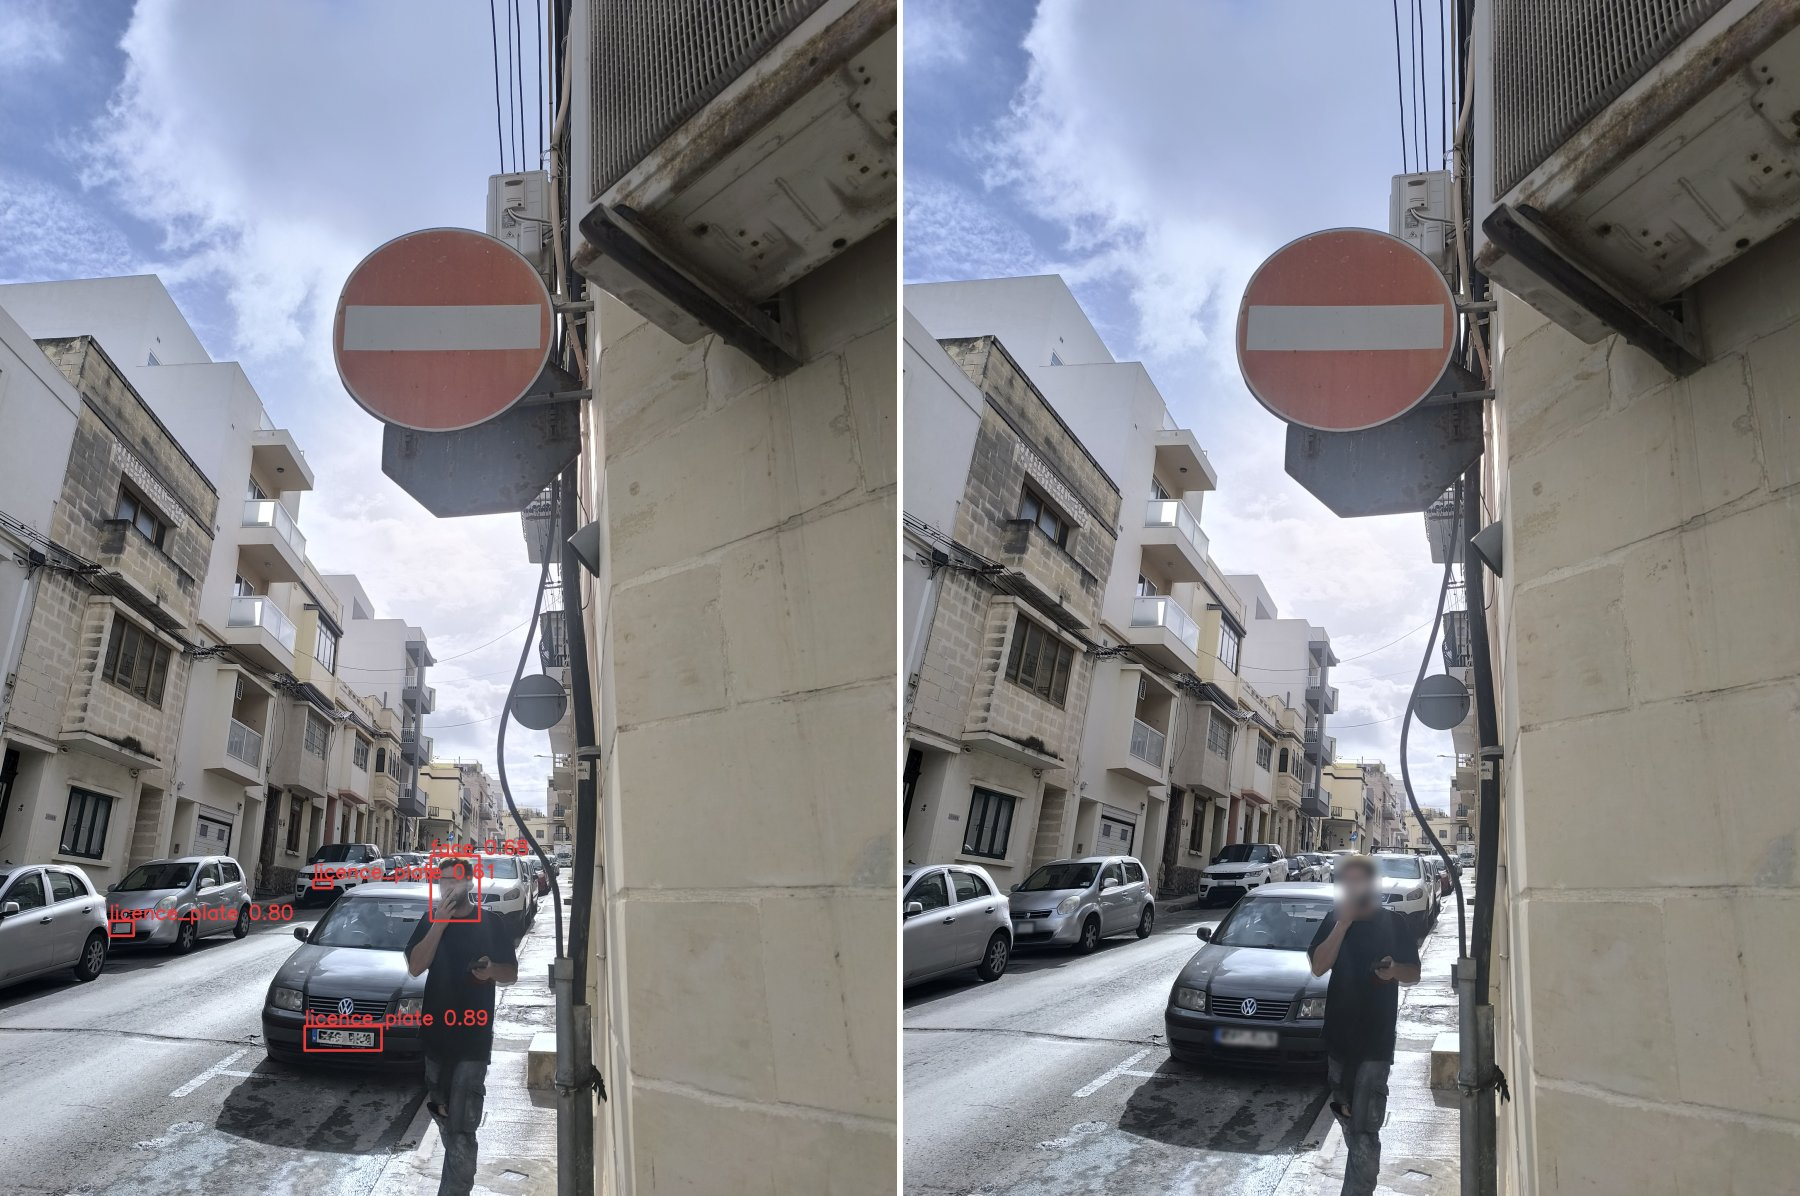
\includegraphics[width=\textwidth]{figures/Anonymization-1.jpg}
    \caption{Automated anonymisation using \gls{SAM} 3.1: predicted privacy regions (left) and the resulting blurred output (right). Faces and registration plates are AI-generated replacements and do not depict the original data.}
    \label{fig:anonymisation-example}
\end{figure}

\subsection{Annotation Procedure and Criteria}
\label{sec:md-annotation-protocol}
Following acquisition and anonymisation, the retained imagery was manually annotated by a team of professional annotators according to the taxonomies and operational definitions established in Chapter~\ref{ch:bg-lit}, supported throughout by dataset-specific guidance promoting consistent interpretation of object categories, inclusion criteria and, for the \gls{MTSD}, the associated object-level attributes. The complete annotation criteria and decision rules are provided in Appendices~\ref{app:mdwd-annotation-criteria} and~\ref{app:mtsd-annotation-criteria}. No model-generated or \gls{AI}-assisted annotations were used. Annotation workflows differed between the two datasets: the \gls{MDWD} was annotated using Roboflow\footnote{\url{https://roboflow.com}}, whereas the \gls{MTSD} was annotated using CVAT\footnote{\url{https://cvat.ai}}, exported in Pascal--VOC XML format, and subsequently consolidated and reviewed using a locally hosted Label Studio\footnote{\url{https://labelstud.io}} instance.

\begin{figure}[H]
    \centering
    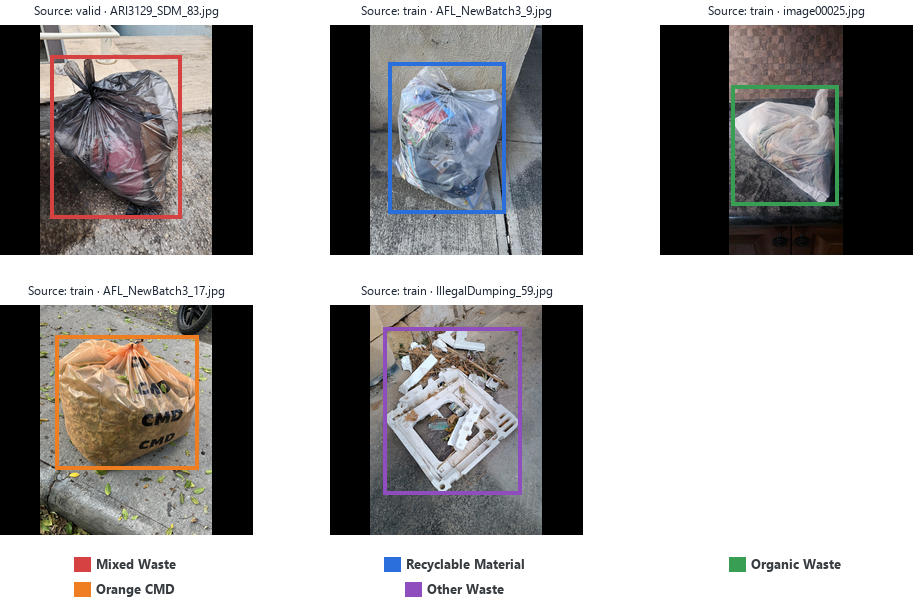
\includegraphics[width=\textwidth]{figures/mdwd_annotation_overview.png}
    \caption{Representative annotated samples illustrating the \gls{MDWD} taxonomy, with bounding-box colours indicating the corresponding waste categories.}
    \label{fig:mdwd-annotation-overview}
\end{figure}
\newpage
\noindent A common bounding-box convention was applied across both datasets, with each annotation tightly enclosing the visible extent of the corresponding object while excluding unrelated background wherever possible, as illustrated for the \gls{MDWD} in Figure~\ref{fig:mdwd-annotation-overview}. Partially occluded objects were retained where approximately \(20\%\) or more remained visible for reliable identification, with boxes restricted to the visible extent rather than extrapolated into occluded regions. Ambiguous or borderline cases were resolved through the review process described in Subsection~\ref{sec:md-annotation-qa}, and the small number of images containing no eligible target objects was retained as negative examples rather than removed from the source corpora.

Similarly, each eligible \gls{MTSD} object was represented by a single bounding box, assigned one traffic-sign category and one label for each of the four object-level attributes, so that all semantic and attribute annotations referred to the same localised instance, as illustrated in Figure~\ref{fig:mtsd-annotation-overview}. Objects were excluded where their identity or required attribute labels could not be established reliably, most commonly when distance, blur, occlusion or poor illumination prevented confident assessment of properties such as geometric shape or physical condition; such exclusions applied only to the affected object, with the surrounding image retained where other valid annotations were present. This avoided introducing uncertain or inferred labels into the \gls{GT} annotations while preserving otherwise usable imagery.

\begin{figure}[H]
    \centering
    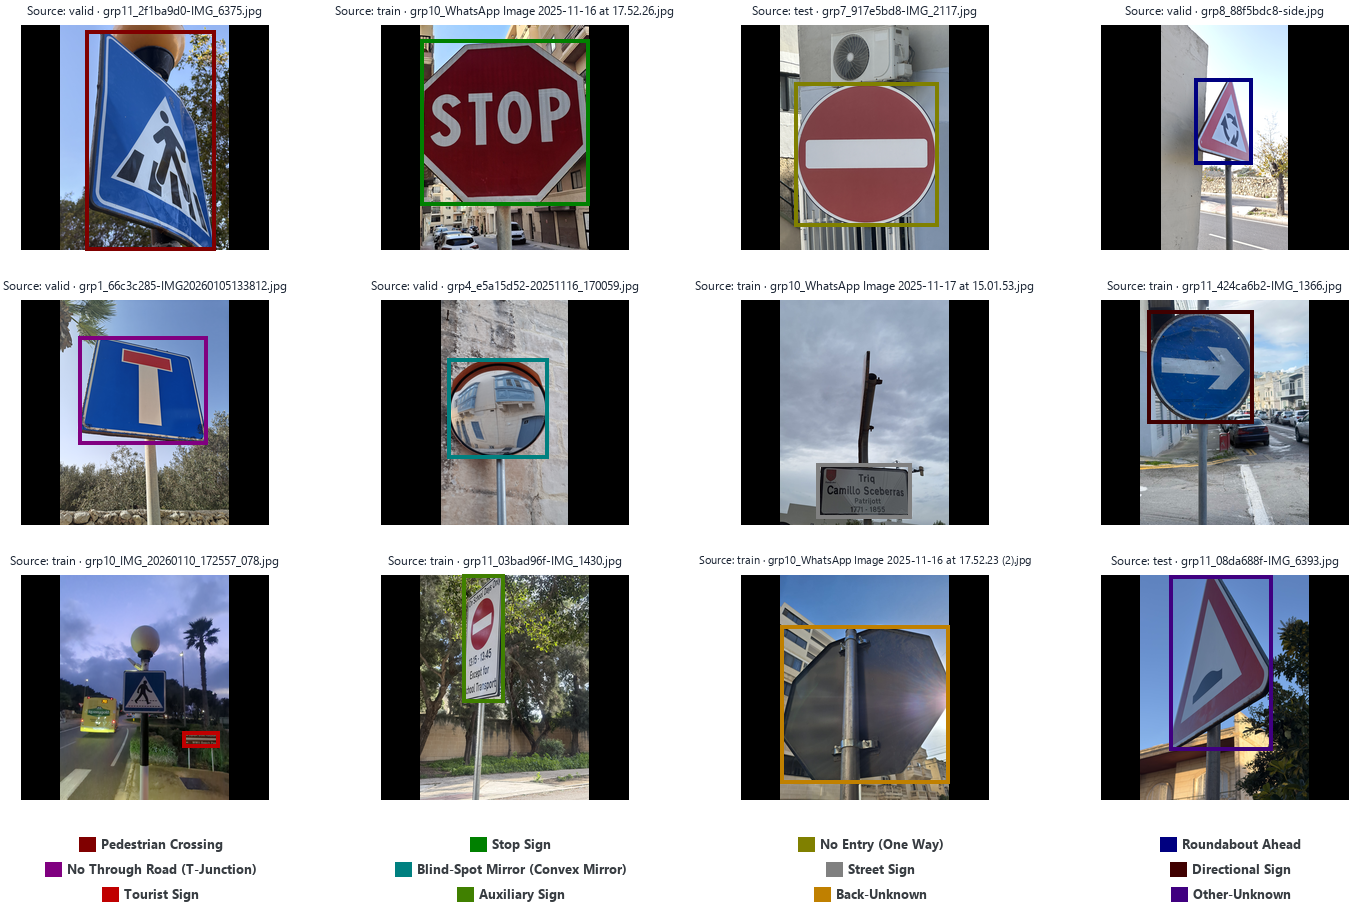
\includegraphics[width=\textwidth]{figures/mtsd_annotation_overview.png}
    \caption{Representative examples of \gls{MTSD} annotations, with one highlighted instance shown for each traffic-sign category.}
    \label{fig:mtsd-annotation-overview}
\end{figure}

\subsection{Annotation \gls{QA} and Agreement Stability Analysis}
\label{sec:md-annotation-qa}
Annotation quality was controlled through the staged review and adjudication workflow illustrated in Figure~\ref{fig:annotation-qa-workflow}, with the objective of establishing a consistent \gls{GT} standard across both datasets. Annotations produced by the annotation team were first examined by the review team and then assessed by the \gls{QA} lead. At this stage, annotations were either accepted as final \gls{GT}, corrected directly by the \gls{QA} lead, or returned to the annotation team where further revision was required. Returned annotations re-entered the workflow from the annotation stage and were reviewed again, with this iterative process continuing until all annotations satisfied the required \gls{QA} standard and were accepted as final \gls{GT}.

\begin{figure}[htbp]
    \centering
    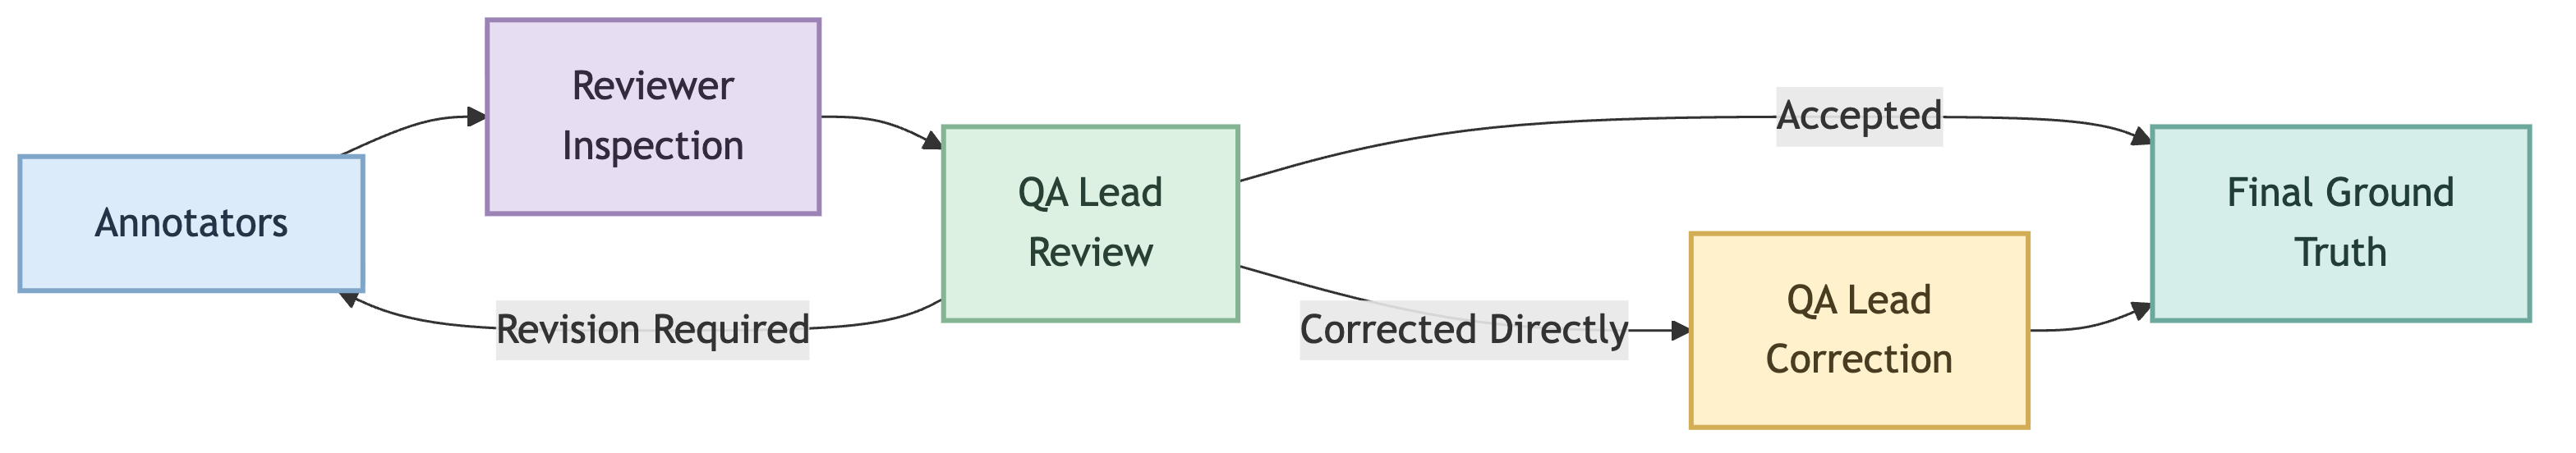
\includegraphics[width=\textwidth]{figures/QA-Workflow.png}
    \caption{Annotation \gls{QA} workflow used to establish the final ground-truth annotations.}
    \label{fig:annotation-qa-workflow}
\end{figure}

\noindent Agreement was quantified using Cohen's \(\kappa\) \cite{cohen1960coefficient} for categorical annotation fields and \gls{IoU} for bounding-box localisation, defined as:

\begin{equation}
\label{eq:kappa-iou}
\kappa = \frac{p_o-p_e}{1-p_e}, \qquad
\mathrm{IoU}(B_1,B_2) = \frac{|B_1\cap B_2|}{|B_1\cup B_2|},
\end{equation}

\noindent where \(p_o\) denotes the observed agreement, \(p_e\) the agreement expected by chance, and \(B_1\) and \(B_2\) the corresponding bounding boxes before and after review.

The versioned annotation history retained for the \gls{MTSD} enabled direct comparison between its initial and reviewed annotation states. Objects were paired within each image using greedy one-to-one matching based on maximum \gls{IoU}, irrespective of class label, with a minimum matching threshold of 0.50. This procedure identified 17,828 matched objects, while 2,681 objects were added and 196 removed during review. Across the matched objects, mean \gls{IoU} reached 0.99, indicating that bounding-box geometry remained highly consistent for instances retained between the two annotation states.

\newpage
\noindent Annotation completeness was considered separately from this geometric agreement. The 2,681 objects introduced during review represent approximately 13.07\% of the 20,509 annotations in the final \gls{MTSD}, indicating that initially omitted instances constituted a more substantial source of correction than bounding-box adjustment. Review also identified recurring revisions to object category, viewing angle and physical condition, together with occasional changes to bounding-box extent. Objects added or removed during review had no corresponding annotation against which agreement could be measured and were therefore excluded from both the mean \gls{IoU} and Cohen's \(\kappa\) calculations.

\begin{table}[h]
\centering
\caption{Agreement between the initial and reviewed \gls{MTSD} annotations for the 17,828 matched objects.}
\label{tab:mtsd-annotation-agreement}
\begin{tabular}{@{}lr@{}}
\toprule
    \textbf{Annotation field} & \textbf{Cohen's $\kappa$} \\
    \midrule
    Object class & 0.97 \\
    Viewing angle & 0.95 \\
    Mounting type & 0.96 \\
    Physical condition & 0.74 \\
    Geometric shape & 0.99 \\
\bottomrule
\end{tabular}
\end{table}

\noindent As shown in Table~\ref{tab:mtsd-annotation-agreement}, most categorical fields remained highly stable through review, with Cohen's \(\kappa\) values between 0.95 and 0.99. The revisions that did occur were concentrated mainly around less clearly defined cases, particularly oblique signs where the boundary between front, side and back views was more difficult to determine, together with occasional corrections between visually or semantically related sign categories. Physical condition exhibited the lowest stability, with a Cohen's \(\kappa\) of 0.74, reflecting the greater interpretative difficulty involved in assessing the severity of visible deterioration. Review frequently required clarification when distinguishing between \emph{Good}, \emph{Weathered} and \emph{Heavily Damaged} signs, particularly where rust, fading, stickers, scratches or minor surface markings were present. This comparatively higher level of revision is therefore taken into account when interpreting the subsequent attribute-classification results.

An equivalent quantitative comparison could not be reproduced for the \gls{MDWD} because its pre-review annotation state was not retained. Qualitative observations from its review process nevertheless indicated that corrections occurred primarily within dense groups of overlapping waste bags, where separating adjacent instances of similar appearance affected both instance identification and bounding-box placement. Some class ambiguity was also observed between recyclable and mixed-waste bags where illumination, discolouration or camera flash altered their apparent colour.

\subsection{Dataset Partitioning and Split Integrity}
\label{sec:md-partitioning}
To preserve independence between model development and evaluation, partitioning was performed at source-corpus level after annotation and \gls{QA}, but before augmentation or any other task-specific transformation. Each dataset was divided into fixed training, validation and test subsets in proportions of \textbf{80/10/10}, without class stratification, balancing or resampling, thereby retaining the naturally occurring class composition of each corpus. The \gls{MDWD} partition was generated once through Roboflow, while the \gls{MTSD} was partitioned deterministically using seed~42, with images sharing identical SHA-256 hashes constrained to the same subset to prevent byte-identical files from crossing partition boundaries. Once established, these source-image assignments were retained throughout the subsequent experiments, providing a consistent basis for training, model selection and final evaluation within each dataset.

\begin{figure}[H]
\centering
    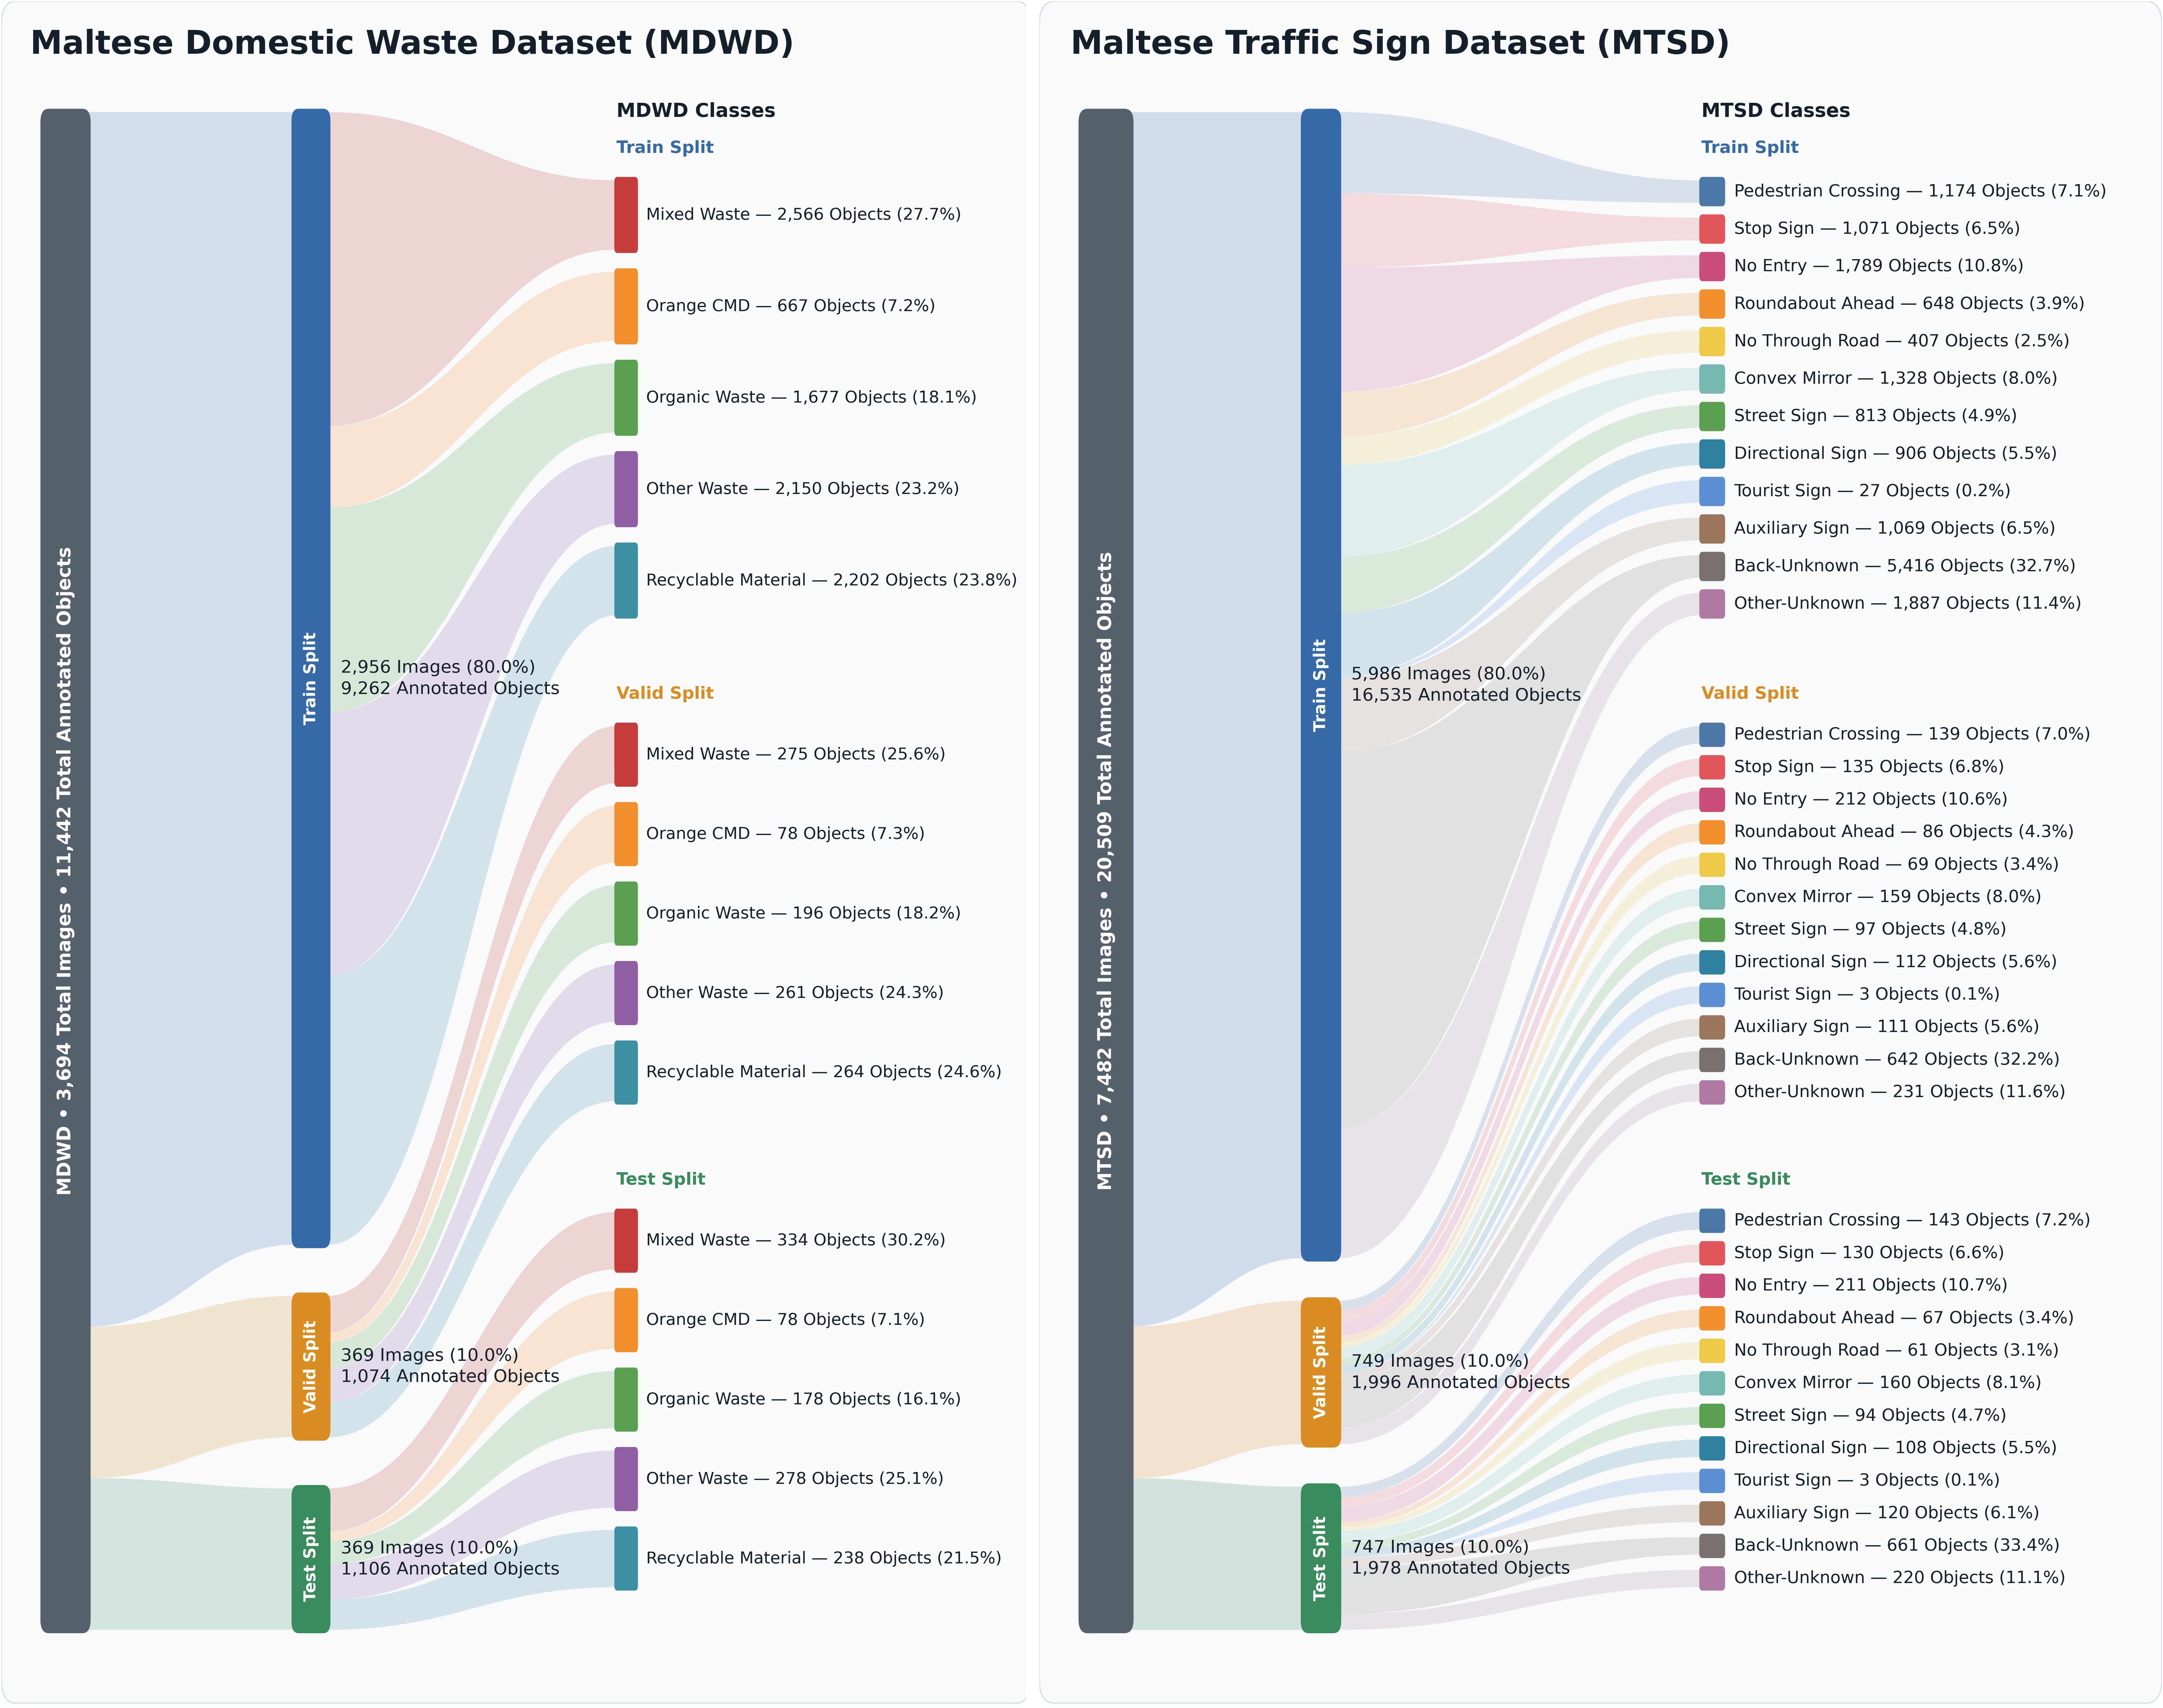
\includegraphics[width=\textwidth]{figures/MDWD-MTSD-Breakdown.png}
    \caption{Training, validation and test partitioning of the \gls{MDWD} and \gls{MTSD}, together with the corresponding class distributions within each split.}
    \label{fig:mdwd-mtsd-breakdown}
\end{figure}

\newpage
\noindent The resulting partition and class distributions, illustrated in Figure~\ref{fig:mdwd-mtsd-breakdown}, show that \gls{MDWD} class proportions remain broadly consistent across the three subsets, varying by less than two percentage points. \emph{Other Waste} is among the more frequently represented categories, reflecting its deliberately heterogeneous scope and inclusion of waste that does not conform to the principal bag-based collection streams. Conversely, \emph{Orange \gls{CMD}} is the least represented class, consistent with the less frequent occurrence of \gls{CMD} cleansing activity relative to routine household waste presentation. Its distinctive colour and presentation nevertheless provide comparatively strong visual separation from the remaining waste categories despite the smaller number of annotated instances.

Greater class imbalance is evident within the \gls{MTSD}, although this arises largely from the structure of the annotation taxonomy rather than from the partitioning procedure itself. \emph{Back-Unknown} constitutes the largest class because conventional traffic signs observed from the rear were assigned to this category whenever their frontal semantic identity could not be established from the available visual evidence. This decision avoided assigning semantic classes through contextual inference or requiring the model to distinguish between sign types that are visually indistinguishable from the rear. Roadside assets whose identity remained recoverable from their physical form, such as convex mirrors and directional bollards, retained their corresponding semantic class irrespective of viewing direction. The prevalence of \emph{Back-Unknown} therefore reflects both the frequency of rear-facing observations and the deliberate treatment of semantic ambiguity within the taxonomy. 

\emph{Other-Unknown} is similarly broad by design, grouping signs outside the explicitly modelled categories rather than fragmenting them into numerous sparsely represented classes. The remaining semantic categories are distributed more consistently across the three partitions, although \emph{Roundabout Ahead} and \emph{No Through Road} show greater proportional variation because of their comparatively small sample sizes.

A further distinction between the source and experiment-ready \gls{MTSD} taxonomies concerns the \emph{Tourist Sign} class. Only 33 instances were present in the source corpus, comprising 27 training, three validation and three test examples, which was considered insufficient for meaningful supervised learning or reliable class-specific evaluation given the visual variability of the category. Its annotations were therefore excluded from the experiment-ready target taxonomy used for supervised detection and zero-shot localisation. The corresponding bounding boxes were retained as ignore regions during localisation evaluation, such that predictions overlapping a Tourist Sign instance were excluded from true-positive and false-positive assignment rather than treated as background errors. This ensured that the class was neither learned nor evaluated as a modelled category while preventing valid localisation of an otherwise recognisable traffic sign from being penalised.

\newpage
\subsection{Exploratory Dataset Analysis (\gls{EDA})}
\label{sec:eda}
The \gls{EDA} was conducted on the final \gls{QA}-approved source annotations to characterise properties of the two datasets likely to influence the subsequent learning tasks, considering object scale, bounding-box geometry and scene density across both corpora, together with \gls{MDWD} class co-occurrence and the distribution of \gls{MTSD} object-level attributes and their association with semantic class. These statistics are calculated across the complete 20,509-instance \gls{MTSD} source corpus, including the 33 \emph{Tourist Sign} instances retained at this stage.

\begin{table}[H]
    \centering
    \caption{Object-scale, bounding-box geometry, and density statistics for both datasets. Relative area denotes bounding-box area as a percentage of the corresponding source-image area.}
    \label{tab:eda-comparison}

    \renewcommand{\arraystretch}{1.15}
    \begin{tabularx}{\textwidth}{@{}Xrr@{}}
        \toprule
        \textbf{Statistic}
        & \textbf{\gls{MDWD}}
        & \textbf{\gls{MTSD}} \\
        \midrule

        \multicolumn{3}{@{}l}{\textit{Object scale}} \\[2pt]
        Relative area, median
            & 2.52\% & 0.94\% \\
        Relative area, Q1--Q3
            & 0.90--5.85\% & 0.03--6.08\% \\
        Objects below 0.1\% of frame
            & 5.81\% & 36.05\% \\

        \midrule
        \multicolumn{3}{@{}l}{\textit{Bounding-box geometry}} \\[2pt]
        Aspect ratio, median
            & 1.00 & 0.91 \\
        Aspect ratio, Q1--Q3
            & 0.80--1.26 & 0.56--1.08 \\

        \midrule
        \multicolumn{3}{@{}l}{\textit{Object density}} \\[2pt]
        Objects per image, mean
            & 3.10 & 2.74 \\
        Objects per image, median
            & 2 & 2 \\
        Objects in busiest image
            & 34 & 24 \\

        \bottomrule
    \end{tabularx}
\end{table}

\noindent As summarised in Table~\ref{tab:eda-comparison}, \gls{MDWD} objects generally occupy a larger proportion of the source image, with a median relative bounding-box area of 2.52\%, compared with 0.94\% for the \gls{MTSD}. The contrast is more pronounced among very small instances, with 36.05\% of \gls{MTSD} objects occupying less than 0.1\% of the source frame, compared with 5.81\% in the \gls{MDWD}. Object density is more comparable between the datasets, averaging 3.10 and 2.74 annotated instances per image, respectively, while the wider interquartile range of \gls{MTSD} aspect ratios reflects greater variation in the geometry of the annotated roadside assets.

\begin{table}[H]
\centering
\caption{Per-class object-scale characteristics for the \gls{MDWD} and \gls{MTSD}. Relative area is expressed as a percentage of the corresponding source-image area.}
\label{tab:eda-class-scale}
\renewcommand{\arraystretch}{1.12}
\small
\begin{tabularx}{\textwidth}{@{}Xrrrr@{}}
\toprule
\textbf{Class} & \textbf{Instances} & \textbf{Q1 (\%)} & \textbf{Median (\%)} & \textbf{$<0.1\%$} \\
\midrule

\multicolumn{5}{@{}l}{\textit{\gls{MDWD}}} \\[2pt]
Mixed Waste             & 3,175 & 1.22 & 3.14 & 2.68\% \\
Orange \gls{CMD}        & 823   & 0.22 & 1.42 & 19.20\% \\
Organic Waste           & 2,051 & 0.88 & 1.84 & 3.46\% \\
Other Waste             & 2,689 & 0.39 & 1.68 & 9.93\% \\
Recyclable Material     & 2,704 & 1.64 & 4.19 & 3.11\% \\

\midrule
\multicolumn{5}{@{}l}{\textit{\gls{MTSD}}} \\[2pt]
Pedestrian Crossing                 & 1,456 & 0.03 & 1.22 & 37.02\% \\
Stop Sign                           & 1,336 & 0.74 & 3.77 & 15.87\% \\
No Entry (One Way)                  & 2,212 & 0.06 & 2.53 & 28.57\% \\
Roundabout Ahead                    & 801   & 0.06 & 3.07 & 29.09\% \\
No Through Road (T-Junction)        & 537   & 2.11 & 4.75 & 7.08\% \\
Blind-Spot Mirror (Convex Mirror)   & 1,647 & 0.40 & 3.88 & 17.30\% \\
Street Sign                         & 1,004 & 0.03 & 0.26 & 41.04\% \\
Directional Sign                    & 1,126 & 0.02 & 0.05 & 62.79\% \\
Tourist Sign                        & 33    & 0.05 & 1.21 & 27.27\% \\
Auxiliary Sign                      & 1,300 & 0.01 & 0.07 & 54.46\% \\
Back-Unknown                        & 6,719 & 0.03 & 0.87 & 37.37\% \\
Other-Unknown                       & 2,338 & 0.02 & 0.13 & 47.35\% \\

\bottomrule
\end{tabularx}
\end{table}

\noindent Considerable variation is also present between semantic classes, as shown in Table~\ref{tab:eda-class-scale}. Within the \gls{MDWD}, \emph{Orange \gls{CMD}} is the smallest category in image space, with a median relative area of 1.42\% and 19.20\% of instances below 0.1\% of the frame. The \gls{MTSD} exhibits substantially greater class-dependent variation: \emph{Directional Sign} has a median relative area of only 0.05\%, with 62.79\% of instances below the 0.1\% threshold, while \emph{Auxiliary Sign}, \emph{Other-Unknown} and \emph{Street Sign} likewise contain particularly high proportions of very small objects. By contrast, classes such as \emph{No Through Road} and \emph{Stop Sign} are typically represented at substantially larger image scales.

\newpage
\noindent Since camera-to-object distance is unavailable within the annotations, relative bounding-box area is used as an image-space proxy for object scale rather than an estimate of physical distance. This provides one basis for interpreting later model behaviour, particularly within the \gls{MTSD}, where the prevalence and class dependence of small objects motivate the input-resolution experiment in Section~\ref{subsec:mtsd-augmentation-resolution}. A complementary source of difficulty arises from the way classes co-occur within individual scenes. Within the \gls{MDWD}, the strongest off-diagonal co-occurrence is observed between \emph{Other Waste} and \emph{Recyclable Material}, which appear together in 589 images, corresponding to 15.94\% of the source corpus. Given the heterogeneous scope of \emph{Other Waste}, this frequent co-occurrence indicates that the detector is often required to distinguish visually competing categories within the same scene. Together, these scale- and context-related characteristics provide the basis for the subsequent robustness analysis in Section~\ref{sec:robustness-error-analysis}.

The four \gls{MTSD} attributes exhibit markedly different class distributions, as illustrated in Figure~\ref{fig:mtsd-attribute-distribution}. Viewing angle is comparatively balanced, whereas mounting type and physical condition are dominated by \emph{Pole-Mounted} and \emph{Good} instances, respectively. Geometric shape is also unevenly distributed, with \emph{Circular} and \emph{Quadrangle} accounting for the majority of annotations and \emph{Pentagon} represented only sparsely. All 20,509 source-corpus instances contain a valid label for each of the four attributes, so this imbalance reflects differences in class prevalence rather than missing supervision.

\begin{figure}[H]
    \centering
    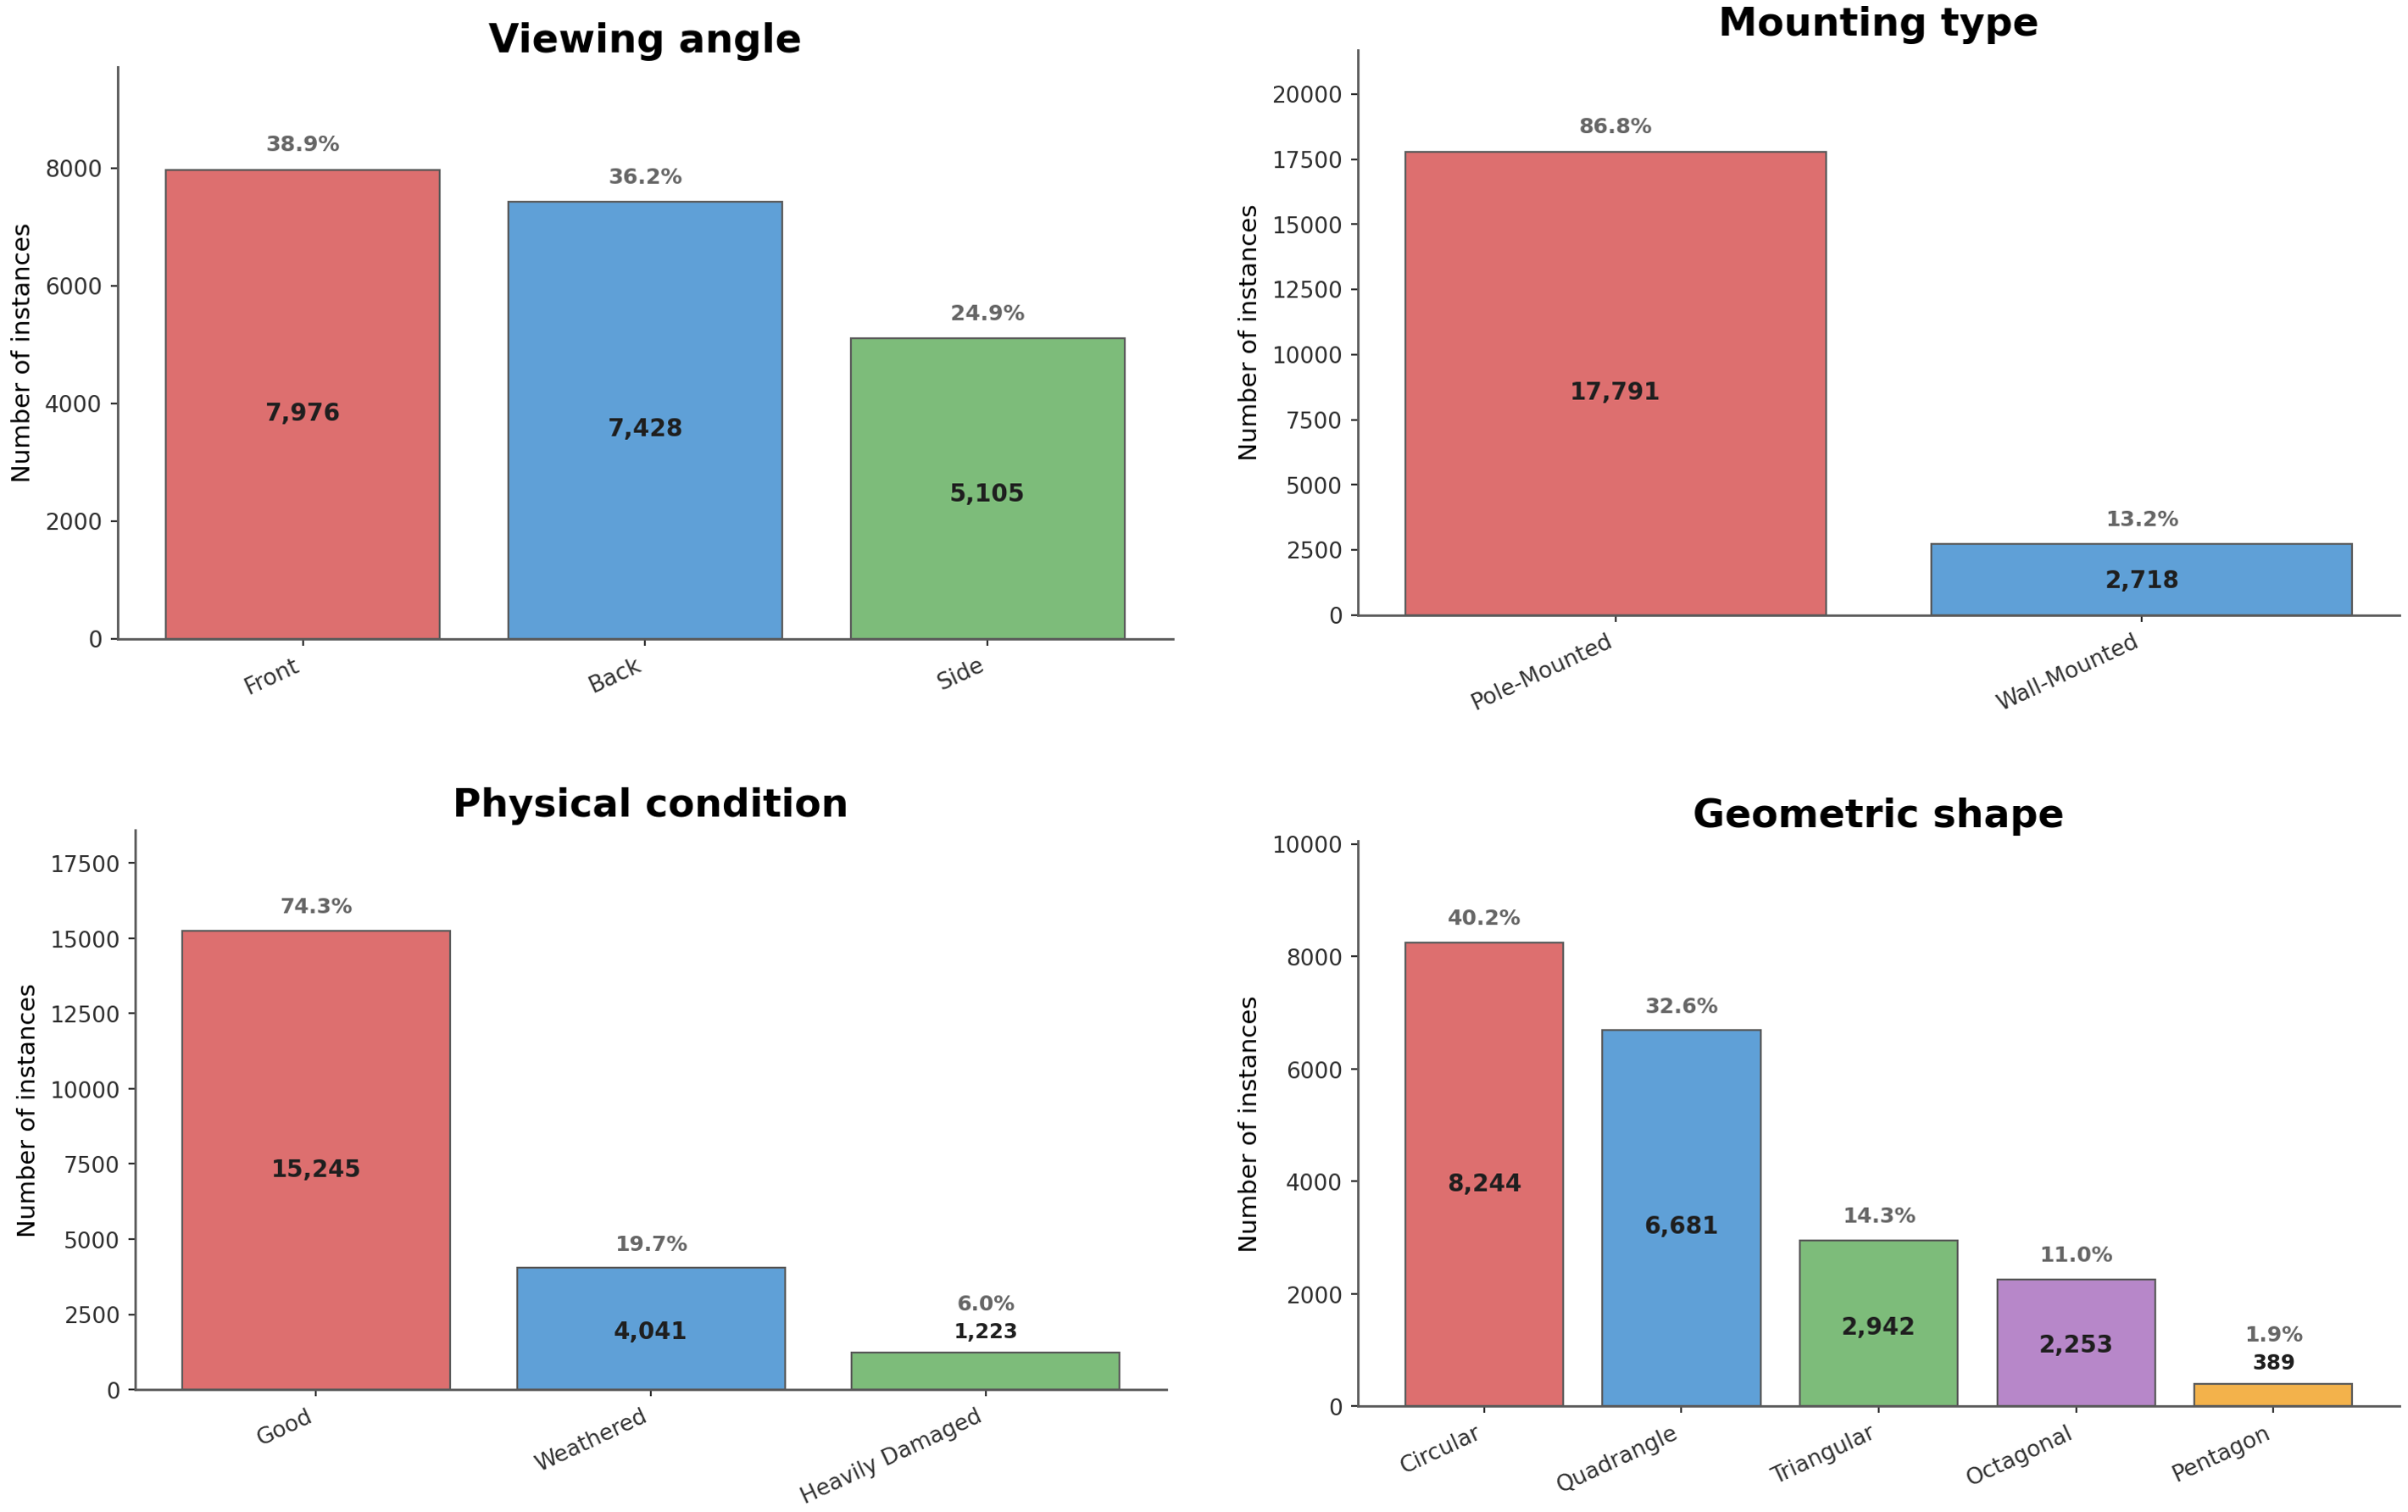
\includegraphics[width=\textwidth]{figures/MTSD_AttributeDistribution.png}
    \caption{Distribution of the four traffic-sign attributes across the 20,509 annotated instances.}
    \label{fig:mtsd-attribute-distribution}
\end{figure}

\noindent Associations between semantic object class and the four \gls{MTSD} attributes were quantified using Cramér's \(V\), which measures association between categorical variables from Pearson's \(\chi^2\) statistic~\cite{cramers}. For a contingency table with \(r\) rows, \(c\) columns and \(n\) observations,

\begin{equation}
\label{eq:cramers-v}
V = \sqrt{\frac{\chi^2}{n\,\min(r-1,c-1)}}.
\end{equation}

\noindent Values range from \(0\), indicating no association, towards \(1\) as association strengthens. Although conventional Cramér's \(V\) can exhibit positive finite-sample bias~\cite{bergsma}, this effect is expected to be limited given the size of the \gls{MTSD} relative to the contingency tables considered. The values are therefore interpreted primarily in terms of relative association strength. As shown in Table~\ref{tab:mtsd-class-attribute-association}, viewing angle and geometric shape exhibit the strongest associations with semantic class, with Cramér's \(V\) values of 0.67 and 0.62, respectively. This reflects the taxonomy, particularly the strong correspondence between \emph{Back-Unknown} and the \emph{Back} viewing-angle label, together with characteristic geometric forms associated with several sign classes. Mounting type shows a moderate association (\(V=0.49\)), driven particularly by the predominance of wall-mounted \emph{Street Sign} instances, while physical condition is only weakly associated with semantic class (\(V=0.14\)).

\begin{table}[H]
\centering
\caption{Association between \gls{MTSD} semantic object class and each object-level attribute, measured using Cramér's \(V\).}
\label{tab:mtsd-class-attribute-association}
\renewcommand{\arraystretch}{1.4}
\setlength{\tabcolsep}{6pt}
\begin{tabularx}{\textwidth}{
    @{}
    >{\raggedright\arraybackslash}p{3.2cm}
    @{\hspace{0.6cm}}
    >{\raggedright\arraybackslash}p{2.2cm}
    @{\hspace{0.6cm}}
    >{\raggedright\arraybackslash}X
    @{}
}
\toprule
\textbf{Attribute} & \textbf{Cramér's \(V\)} & \textbf{Principal association} \\
\midrule
Viewing angle      & 0.67 & \emph{Back-Unknown} strongly associated with \emph{Back} \\
Mounting type      & 0.49 & \emph{Street Sign} predominantly wall-mounted \\
Physical condition & 0.14 & Weak association with semantic class \\
Geometric shape    & 0.62 & Strong class-specific geometric structure \\
\bottomrule
\end{tabularx}
\end{table}

\noindent These relationships are relevant to the subsequent attribute-classification experiments, since some attributes may be predicted partly from cues associated with semantic identity, while physical condition depends more directly on the observed state of the individual asset. Attribute imbalance is therefore considered through overall accuracy, macro-averaged \(F_1\) and per-class measures.

\subsection{Experimental Data Preparation and Augmentation}
\label{sec:md-training-data-prep}
Following the source-image partitioning defined in Subsection~\ref{sec:md-partitioning}, data preparation was performed separately for each experimental track while preserving validation and test independence. Augmentation was restricted to the training data, with held-out images receiving only model-specific deterministic preprocessing. The \gls{MDWD} detection experiments used a fixed offline augmentation pipeline, whereas the \gls{MTSD} detection experiments compared three augmentation strategies. Attribute classification employed a separate crop-based pipeline with online training augmentation.

\subsubsection{\gls{MDWD} Detection Data Preparation and Augmentation}
\label{sec:md-augmentation-mdwd}
The \gls{MDWD} imagery was first normalised to a consistent orientation and subsequently resized to \(640 \times 640\) pixels using stretch-based resizing. Preliminary resolution trials produced only marginal differences in validation performance across the tested input sizes, indicating that the standard \(640 \times 640\) configuration provided an appropriate balance between predictive performance and computational cost. This resolution was therefore retained as the fixed reference input size for all \gls{MDWD} detector experiments, ensuring that all models were trained and evaluated under a common spatial configuration.

Stretch-based resizing was selected in preference to letterboxing to avoid introducing padding that could interact with the subsequent mosaic augmentation process. Because the source imagery is predominantly portrait-oriented, resizing directly to a square input alters the original aspect ratio and introduces anisotropic geometric distortion. However, this transformation was applied consistently across the complete \gls{MDWD} and was therefore treated as part of the standardised experimental representation rather than as a source of variation between detector configurations.

Offline augmentation was generated once using Roboflow and reused across all \gls{MDWD} detector experiments to ensure a consistent training corpus. Ten outputs were produced per source training image, consisting of the resized original and nine augmented derivatives, increasing the effective training set to 29,580 images. Generating the augmented corpus in advance ensured that each detector was exposed to the same transformed samples, supporting a fair comparison across architectures. All augmentation was restricted to the training partition, while validation and test imagery remained unchanged apart from the required deterministic preprocessing. The applied transformations and their respective configurations are summarised in Table~\ref{tab:mdwd-augmentation}.

\begin{table}[H]
  \caption{Offline augmentation configuration applied to the \gls{MDWD} training partition through Roboflow.}
  \label{tab:mdwd-augmentation}
  \centering
  \begin{tabular*}{\columnwidth}{@{\extracolsep{\fill}}lr@{}}
    \toprule
    \textbf{Augmentation} & \textbf{Configuration} \\
    \midrule
    Resize                & $640 \times 640$ (Stretch) \\
    Horizontal Flip       & 50\% probability \\
    Vertical Flip         & 50\% probability \\
    Hue Adjustment        & $\pm 19^{\circ}$ \\
    Saturation Adjustment & $\pm 29\%$ \\
    Brightness Adjustment & $\pm 17\%$ \\
    Exposure Adjustment   & $\pm 10\%$ \\
    Gaussian Blur         & Up to 1\,px \\
    Motion Blur           & Up to 40\,px \\
    Mosaic Augmentation   & Enabled ($2{\times}2$) \\
    \bottomrule
  \end{tabular*}
\end{table}

\noindent The selected transformations were chosen to reflect variation expected during street-level image acquisition, with representative augmented samples shown in Figure~\ref{fig:mdwd-augmentation-examples}. Photometric augmentation broadens variation in illumination, colour and image response, while Gaussian and motion blur simulate degradation associated with imperfect focus and camera or vehicle movement. Mosaic augmentation further increases diversity in surrounding context, apparent object scale and spatial arrangement by combining multiple training images into a single composite sample.

\begin{figure}[H]
    \centering
    \makebox[\textwidth][c]{%
        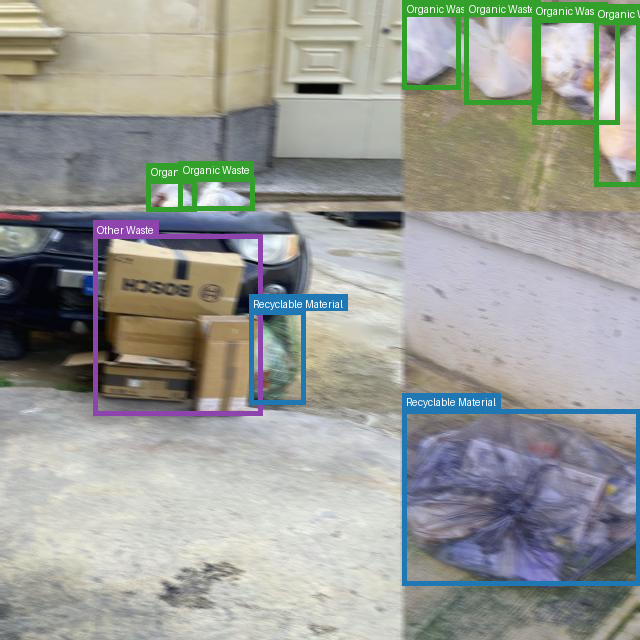
\includegraphics[width=0.5\textwidth]{figures/MDWD-Aug-1.jpg}%
        \hspace{0.02\textwidth}%
        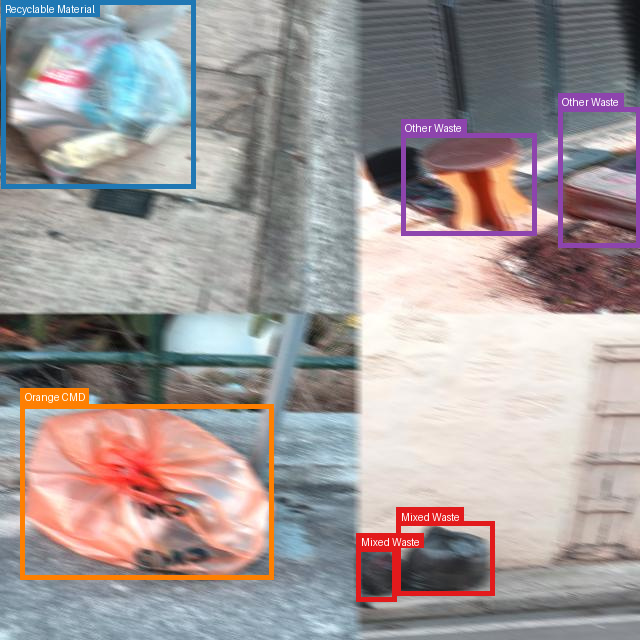
\includegraphics[width=0.5\textwidth]{figures/MDWD-Aug-2.jpg}%
    }
    \caption{Two representative examples of the final augmented \gls{MDWD} training images supplied to the detection models, illustrating the combined augmentation pipeline with overlaid bounding boxes denoting annotated \gls{MSW} instances.}
    \label{fig:mdwd-augmentation-examples}
\end{figure}

\newpage
\noindent Horizontal reflection was retained as a conventional augmentation for street-level imagery, while vertical reflection was included specifically for the \gls{MDWD} due to the less constrained orientation of deformable waste objects, which may topple, collapse or otherwise appear in irregular configurations. Motion blur of up to 40 pixels was also applied to reflect acquisition artefacts observed in imagery captured from slowly moving vehicles. Although comparatively aggressive, this transformation was retained because preliminary validation indicated improved generalisation.

\subsubsection{\gls{MTSD} Detection Augmentation Strategies}
\label{sec:md-augmentation-mtsd}
To examine the effect of training-data variation on \gls{MTSD} detection performance, three alternative augmentation strategies were defined: \emph{none}, \emph{mild} and \emph{strong}. All three operate from the same fixed source-image partitions, comprising 5,986 training, 749 validation and 747 test images, so that the experimental conditions differ in their training representations rather than their underlying data allocation. The \emph{none} strategy provides the unaugmented reference condition using the original \gls{QA}-approved imagery, while \emph{mild} and \emph{strong} each generate four outputs per source training image, consisting of the original and three augmented derivatives, expanding the training set from 5,986 to 23,944 images. The two strategies progressively increase the degree of visual variation presented during training, as illustrated comparatively in Figure~\ref{fig:mtsd-augmentation-examples}.

\begin{figure}[H]
    \centering
    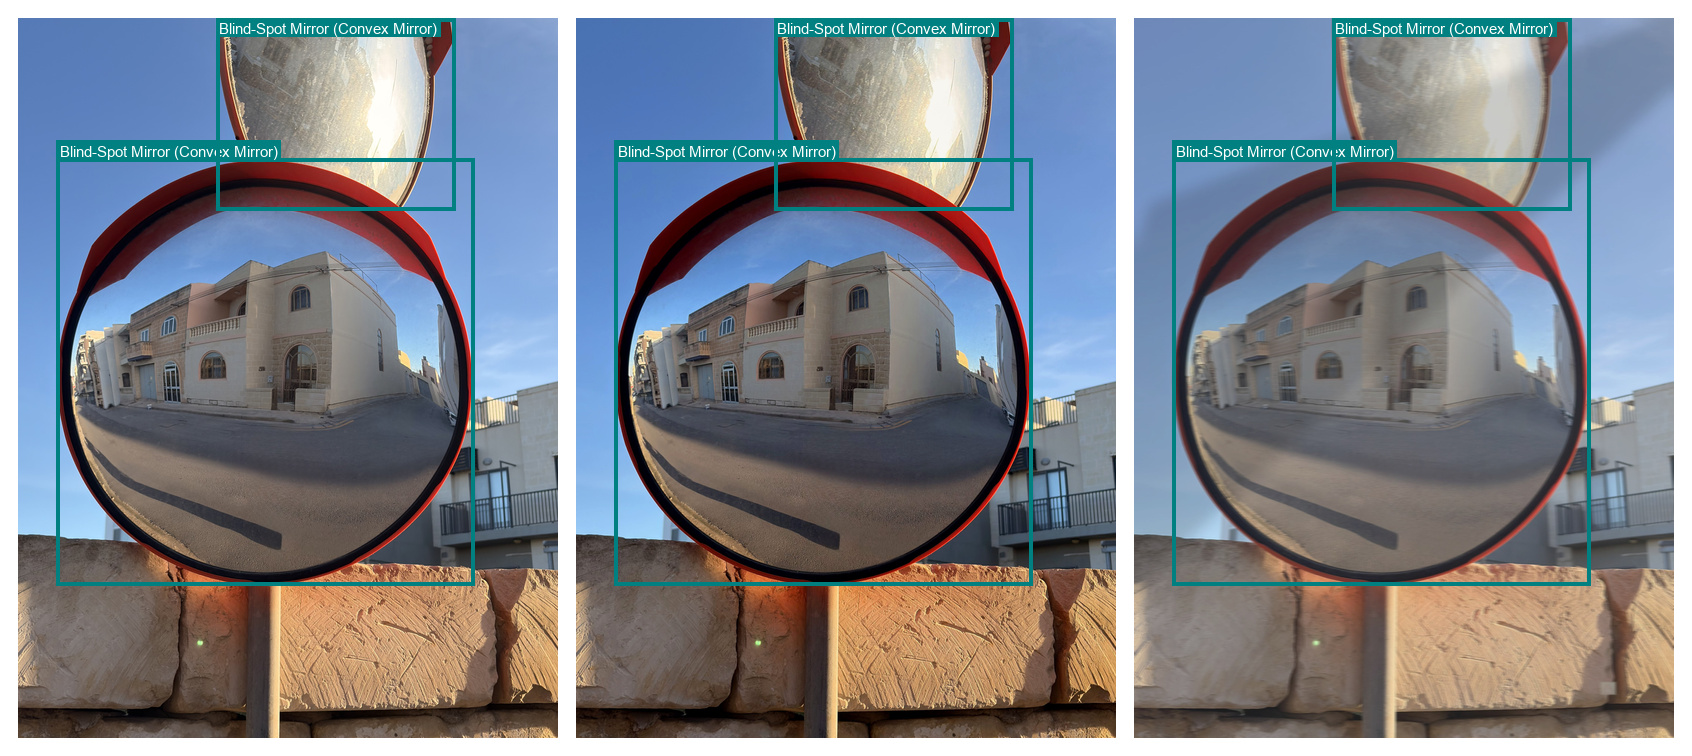
\includegraphics[width=\textwidth]{figures/MTSD-Aug-1.jpg}
    \caption{Representative \gls{MTSD} sample under the three augmentation strategies: \emph{none} (left), \emph{mild} (centre) and \emph{strong} (right), illustrating the progressively greater photometric and geometric variation introduced by each strategy.}
    \label{fig:mtsd-augmentation-examples}
\end{figure}

\newpage
\noindent The \emph{mild} strategy was designed to preserve object geometry and bounding-box coordinates while introducing limited photometric and acquisition-related variation. The transformation ranges reported in Table~\ref{tab:mtsd-augmentation} were therefore selected to produce modest departures from the source imagery, broadening visual appearance without substantially altering the spatial characteristics of the traffic signs.

By contrast, the \emph{strong} strategy introduces broader geometric and scene-level variation, including changes to object position, scale, orientation and perspective, together with more substantial modifications to illumination and scene composition. Where a transformation alters object geometry or visibility, the associated bounding boxes are recalculated, clipped to the visible image region and filtered according to the criteria in Table~\ref{tab:mtsd-augmentation}. The strategy was designed to expose detectors to a wider range of plausible viewing and acquisition conditions while preserving the semantic identity of the underlying traffic sign.

\begin{table}[h]
\centering
\caption{Offline augmentation configurations for the \emph{mild} and \emph{strong} \gls{MTSD} strategies.}
\label{tab:mtsd-augmentation}

\normalsize
\renewcommand{\arraystretch}{1.04}
\setlength{\tabcolsep}{4pt}

\begin{tabularx}{\textwidth}{
    @{}
    >{\raggedright\arraybackslash}p{3.4cm}
    >{\raggedright\arraybackslash}p{4.3cm}
    >{\raggedright\arraybackslash}X
    @{}
}
\toprule
\textbf{Transformation} & \textbf{Mild} & \textbf{Strong} \\
\midrule

Brightness
& \(0.80\)--\(1.20\)
& \(75\%\), \(0.65\)--\(1.35\) \\

Contrast
& \(0.85\)--\(1.15\)
& \(75\%\), \(0.70\)--\(1.30\) \\

Saturation
& \(0.90\)--\(1.10\)
& \(70\%\), \(0.80\)--\(1.20\) \\

Gamma
& \(0.90\)--\(1.10\)
& \(70\%\), \(0.70\)--\(1.35\) \\

\addlinespace[0.15em]

Gaussian blur
& \(50\%\), \(\sigma \leq 1.0\)
& \(50\%\), \(\sigma \leq 1.5\) \\

Gaussian noise
& \(30\%\), \(\sigma \leq 0.02\)
& \(50\%\), \(\sigma \leq 0.04\) \\

JPEG compression
& \(30\%\), quality \(70\)--\(92\)
& \(60\%\), quality \(45\)--\(90\) \\

Motion blur
& Horizontal \(9\)-px kernel, weight \(0.85\)
& \(35\%\), kernel \(\{7,9,11\}\) px \\

\addlinespace[0.15em]

Illumination effects
& --
& Shadow \(25\%\); gradient \(25\%\); local \(20\%\); haze \(15\%\) \\

Translation
& --
& Up to \(10\%\) width/height \\

Scale
& --
& \(0.75\)--\(1.30\) \\

Rotation
& --
& \(-5^{\circ}\) to \(+5^{\circ}\) \\

Shear
& --
& Up to \(2^{\circ}\) \\

Perspective
& --
& Distortion \(0.02\) \\

Random crop
& --
& \(35\%\); retained-box visibility \(\geq 85\%\) \\

\addlinespace[0.15em]

Mosaic
& --
& \(40\%\); \(1280 \times 1280\); centre \(40\%\)--\(60\%\) \\

Rare-class copy-paste
& --
& \(20\%\); up to 2 instances; scale \(0.80\)--\(1.25\); max.\ \gls{IoU} \(0.20\) \\

\addlinespace[0.15em]

Bounding-box handling
& Coordinates unchanged
& Recomputed and filtered: visibility \(\geq 35\%\), dimensions \(\geq 2\) px, area \(\geq 9\) px \\

\midrule

\textbf{Training-set size}
& \textbf{23,944 images}
& \textbf{23,944 images} \\

\bottomrule
\end{tabularx}
\end{table}

\newpage
\noindent To complement this broader augmentation strategy, rare-class copy-paste was applied to increase the representation of underrepresented modelled categories, particularly \emph{Roundabout Ahead} and \emph{No Through Road}. Up to two annotated instances were inserted subject to predefined scale and overlap constraints, with source identity, placement coordinates and resulting bounding boxes recorded in the augmentation manifest for reproducibility. Consequently, the \emph{strong} strategy modifies not only the visual diversity of the training data, but also its effective class distribution, as quantified in Table~\ref{tab:mtsd-augmentation-class-balance}.

\begin{table}[H]
\centering
\caption{Effective \gls{MTSD} training-instance counts under the three augmentation strategies.}
\label{tab:mtsd-augmentation-class-balance}
\small
\begin{tabularx}{\textwidth}{@{}Xrrr@{}}
\toprule
\textbf{Class} & \textbf{None} & \textbf{Mild} & \textbf{Strong} \\
\midrule
Pedestrian Crossing & 1,174 & 4,696 & 8,635 \\
Stop Sign & 1,071 & 4,284 & 7,998 \\
No Entry (One Way) & 1,789 & 7,156 & 13,048 \\
Roundabout Ahead & 648 & 2,592 & 6,519 \\
No Through Road (T-Junction) & 407 & 1,628 & 4,827 \\
Blind-Spot Mirror (Convex Mirror) & 1,328 & 5,312 & 9,863 \\
Street Sign & 813 & 3,252 & 5,823 \\
Directional Sign & 906 & 3,624 & 6,296 \\
Auxiliary Sign & 1,069 & 4,276 & 7,562 \\
Back-Unknown & 5,416 & 21,664 & 39,519 \\
Other-Unknown & 1,887 & 7,548 & 13,624 \\
\midrule
\textbf{Modelled total} & \textbf{16,508} & \textbf{66,032} & \textbf{123,714} \\
\bottomrule
\end{tabularx}
\end{table}

\noindent Across the 11 modelled classes, the majority-to-minority ratio remains unchanged at 13.31 under the \emph{none} and \emph{mild} strategies, but decreases to 8.19 under \emph{strong}. The corresponding coefficient of variation also falls from 0.87 to 0.83, indicating a modest reduction in overall class-frequency dispersion. Horizontal reflection was excluded because it may alter semantically meaningful sign orientation, while MixUp was omitted because translucent composites were considered unrepresentative of plausible street-level observations. All offline augmentation was generated deterministically from seed~42, source-image identity and derivative index, ensuring that the experiment-ready corpora can be reproduced consistently.

The three conditions are therefore treated as complete training-data strategies rather than as a single-factor augmentation ablation. They differ in both the extent of introduced variation and the resulting training exposure, with the \emph{strong} strategy additionally affecting object geometry, scene composition and class balance. Subsequent performance differences are consequently interpreted at the strategy level rather than attributed to individual transformations.

\subsubsection{Attribute-Crop Generation and Online Augmentation}
\label{sec:md-augmentation-attribute}
Attribute classification uses an object-centred representation derived directly from the \gls{GT} annotations of the \gls{MTSD}. Each annotated instance was extracted with a \(25\%\) contextual margin around its bounding box, retaining limited surrounding scene information that may support interpretation of attributes such as mounting type and viewing angle, and square-padded with neutral grey rather than geometrically stretched, preserving the sign's original proportions prior to model-specific resizing and normalisation. Figure~\ref{fig:mtsd-attribute-crop-preparation} illustrates this preparation process, from the annotated source image through contextual expansion to the resulting square-padded model input. A single crop was generated per annotated instance, with no offline augmentation applied during crop generation.

\begin{figure}[H]
    \centering
    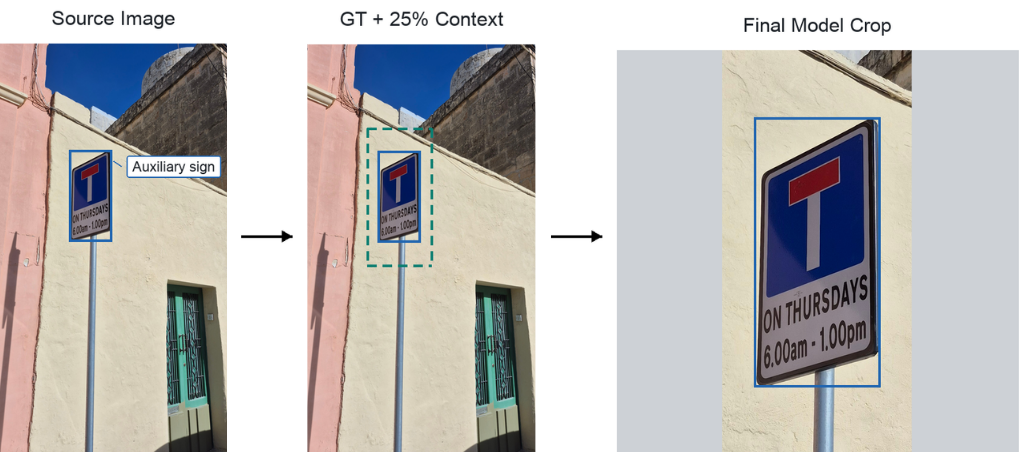
\includegraphics[width=\textwidth]{figures/MTSD-AttrCls.png}
    \caption{Attribute-crop preparation from the \gls{MTSD} source imagery, showing the \gls{GT} object localisation, \(25\%\) contextual expansion and square-padded model input.}
    \label{fig:mtsd-attribute-crop-preparation}
\end{figure}

\noindent Rather than generating additional crop variants offline, augmentation was applied dynamically to training crops only, while validation and test crops followed a fixed, deterministic pipeline. Training crops were first square-padded with the neutral-grey fill value \((114,114,114)\) and randomly rotated within \(\pm10^\circ\), with regions exposed by rotation filled with the same neutral grey. A \texttt{RandomResizedCrop} then sampled \(80\text{--}100\%\) of the padded area at an aspect ratio of \(0.90\text{--}1.11\), resizing the result to the backbone-specific resolution with antialiasing. Colour jitter was applied last, perturbing brightness and contrast by up to \(0.3\), saturation by up to \(0.2\), and hue by up to \(0.02\), before tensor conversion and ImageNet normalisation. Horizontal reflection was deliberately excluded, as it may alter orientation-dependent cues relevant to sign content and viewing angle, and no other transformations were applied. Validation and test crops, by contrast, underwent only square padding, antialiased resizing, tensor conversion and normalisation, with no rotation, cropping or colour perturbation, ensuring a consistent and reproducible evaluation input.

\newpage 
\section{Supervised Object Detection (\gls{OD})} 
\label{sec:supervised-detection-methodology}
The supervised detection study compares \gls{YOLO}11, \gls{YOLO}12, \gls{YOLO}26 and \gls{RF-DETR} across both the \gls{MDWD} and \gls{MTSD}, following the architectural rationale established in Section~\ref{sec:bg-supervised-od}. The methodology focuses on how detector family, model scale, training-data strategy and input resolution influence predictive performance and computational requirements under a common experimental framework. Each configuration was trained and evaluated using fixed dataset partitions, with task-specific weights learned independently for the two municipal domains. The following subsections define the model-scale comparisons, pretrained initialisation, shared training configuration and the additional augmentation and resolution experiments conducted on the \gls{MTSD}.

\subsection{Model-Scale Experiments}
\label{sec:supervised-model-ablation}
Each detector family was evaluated across multiple model scales to examine how increasing model capacity influences both predictive performance and computational demand. The principal comparison comprises the Nano (-N), Small (-S) and Medium (-M) variants of \gls{YOLO}11, \gls{YOLO}12, \gls{YOLO}26 and \gls{RF-DETR}, with the Large (-L) configuration additionally included for \gls{YOLO}26. Collectively, these variants form the 13 detector configurations summarised in Table~\ref{tab:model-matrix}.

Each configuration was trained independently on the \gls{MDWD} and \gls{MTSD}, with no transfer of task-specific weights between domains. Fixed dataset partitions were retained throughout so that within-dataset differences between model families and scales were assessed against an identical held-out test set.

\begin{table}[htbp]
\centering
\caption{Supervised detector families and model scales evaluated on the \gls{MDWD} and \gls{MTSD}. Parameter counts refer to the corresponding published pretrained detection checkpoints and are reported in millions of parameters.}
\label{tab:model-matrix}
\renewcommand{\arraystretch}{1.16}
\small
\begin{tabularx}{\textwidth}{
@{}
>{\raggedright\arraybackslash}p{2.1cm}
>{\raggedright\arraybackslash}X
>{\centering\arraybackslash}p{1.25cm}
>{\centering\arraybackslash}p{1.25cm}
>{\centering\arraybackslash}p{1.25cm}
>{\centering\arraybackslash}p{1.25cm}
@{}
}
\toprule
\textbf{Family} & \textbf{Architectural emphasis} & \textbf{N} & \textbf{S} & \textbf{M} & \textbf{L} \\
\midrule
\multicolumn{6}{@{}l}{\textit{\gls{YOLO}-based detectors}} \\
\addlinespace[0.2em]
    \gls{YOLO}11 & Efficiency-oriented \gls{YOLO} baseline & 2.6\,M & 9.4\,M & 20.1\,M & -- \\
    \gls{YOLO}12 & Attention-centric \gls{YOLO} & 2.6\,M & 9.3\,M & 20.2\,M & -- \\
    \gls{YOLO}26 & End-to-end, edge-oriented \gls{YOLO} & 2.4\,M & 9.5\,M & 20.4\,M & 24.8\,M \\
    \midrule
    \multicolumn{6}{@{}l}{\textit{Detection transformer}} \\
    \addlinespace[0.2em]
    \gls{RF-DETR} & \gls{DINO}v2-based detection transformer & 30.5\,M & 32.1\,M & 33.7\,M & -- \\
\bottomrule
\end{tabularx}
\end{table}

\newpage
\noindent Within each family, the -N variant represents the lowest-capacity configuration, while the -S and -M variants progressively increase model capacity at the cost of additional memory and computation. Comparing these scales therefore indicates whether increased capacity produces corresponding improvements in predictive performance or begins to yield diminishing returns. The \gls{YOLO}26-L configuration is not intended as a common scale across families, but is used specifically to examine whether this newest, deployment-oriented \gls{YOLO} architecture continues to benefit from increased capacity beyond -M.

The scale designations are interpreted within each detector family rather than as equivalent parameter budgets across architectures. For example, \gls{RF-DETR}-N contains substantially more parameters than the corresponding \gls{YOLO}-N models, while the increase in parameter count between its -N and -M variants is considerably smaller. The within-family comparisons therefore form the model-capacity analysis, while comparisons between detector families are treated as practical architecture-level comparisons rather than parameter-matched experiments.

\subsection{Pretrained Initialisation and Training Provenance}
\label{sec:supervised-pretraining-provenance}
All supervised detectors were fine-tuned from pretrained weights rather than trained from random initialisation. Checkpoint provenance is reported explicitly because differences in upstream pretraining form part of the conditions under which the resulting models are compared. Table~\ref{tab:detector-pretraining} summarises the initialisation checkpoint, pretraining provenance and training environment used for each configuration.

\begin{table}[htbp]
\centering
\caption{Pretrained initialisation and training provenance of the supervised detector configurations.}
\label{tab:detector-pretraining}
\renewcommand{\arraystretch}{1.25}
\small
\begin{tabularx}{\textwidth}{ @{}
>{\raggedright\arraybackslash}p{1.6cm}
>{\raggedright\arraybackslash}p{3.8cm}
>{\raggedright\arraybackslash}p{2.4cm}
>{\raggedright\arraybackslash}X
>{\raggedright\arraybackslash}p{2.4cm} @{} }
\toprule
\textbf{Family} & \textbf{Initialisation checkpoint} & \textbf{Checkpoint provenance} & \textbf{Dataset} & \textbf{Training} \\
\midrule
\gls{YOLO}11 & \texttt{yolo11\{n,s,m\}.pt} & \gls{COCO} & \gls{MDWD} and \gls{MTSD} & Local workstation \\
\gls{YOLO}12 & \texttt{yolo12\{n,s,m\}.pt} & \gls{COCO} & \gls{MDWD} and \gls{MTSD} & Local workstation \\
\gls{YOLO}26 & \texttt{yolo26\{n,s,m,l\}.pt} & Objects365 \& \gls{COCO}\textsuperscript{\dag} & \gls{MDWD} and \gls{MTSD} & Local workstation \\
\midrule
\gls{RF-DETR} & \texttt{rf-detr-\{n,s,m\}.pth} & Objects365 \& \gls{COCO}\textsuperscript{\dag} & \gls{MDWD} (-N) and \gls{MTSD} & Local workstation \\
\gls{RF-DETR} & Roboflow-hosted checkpoint & Objects365 \& \gls{COCO}\textsuperscript{*} & \gls{MDWD} (-S and -M) & Roboflow hosted \\
\bottomrule
\end{tabularx}
\vspace{0.4em}
\begin{minipage}{0.97\textwidth}
\footnotesize
\textsuperscript{\dag}Released checkpoints are pretrained on Objects365 and subsequently fine-tuned on \gls{COCO} \cite{hidayatullah2026yolo26, robinson2026rfdetrneuralarchitecturesearch}.\\
\textsuperscript{*}Objects365-pretrained checkpoint intialised from Roboflow platform.
\end{minipage}
\end{table}

\newpage
\noindent With the exception of the \gls{MDWD} \gls{RF-DETR}-S and -M configurations, all supervised detectors were trained locally on a workstation equipped with an AMD Ryzen~9 7900X3D processor, 128\,GB of \gls{DDR5} memory and a single NVIDIA RTX~4090 \gls{GPU} with 24\,GB of memory. Training runs were tracked using Weights~\&~Biases\footnote{\url{https://wandb.ai/}}. The local software environment comprised Python~3.12.13, Ultralytics~8.4.101, \gls{RF-DETR}~1.3.0 and Transformers~4.57.6, with PyTorch~2.10.0 (nightly build) and \gls{CUDA}~13.0. Framework-specific dependencies were isolated where required, while the same hardware and fixed dataset partitions were retained across all locally trained experiments.

The computational requirements of \gls{RF-DETR}-S and -M on the augmented \gls{MDWD} training corpus made local training impractical within the available timeframe, and these two configurations were instead trained on the Roboflow hosted platform. The same fixed \gls{MDWD} partitions and experiment-ready representation were retained throughout. The \gls{MDWD} \gls{RF-DETR} scale comparison therefore reflects a minor variation in initialisation and training environment alongside model capacity, whereas the \gls{MTSD} \gls{RF-DETR} comparison is unaffected, as all three scales used the same released checkpoints and local configuration.

\subsection{Shared Training Hyperparameters}
\label{sec:supervised-hyperparams}
A common training configuration was adopted for the locally trained supervised \glspl{OD} across both datasets. The hyperparameters summarised in Table~\ref{tab:hyperparams} were held constant wherever supported, providing a consistent optimisation basis for comparing detector configurations. The \gls{RF-DETR}-S and -M configurations trained through Roboflow followed the same training-duration and early-stopping criteria, while their remaining optimisation settings followed the platform defaults.

Input resolution was treated independently from the shared configuration. All \gls{MDWD} detectors used the fixed \(640 \times 640\)-pixel stretch-based representation established in Subsection~\ref{sec:md-augmentation-mdwd}, whereas resolution was retained as an experimental factor for the \gls{MTSD}, examined together with the augmentation strategies in Subsection~\ref{subsec:mtsd-augmentation-resolution}.

\begin{table}[H]
\caption{Shared training hyperparameters used for locally trained supervised detectors.}
\label{tab:hyperparams}
\centering
\begin{tabular*}{\columnwidth}{@{\extracolsep{\fill}}lr@{}}
\toprule
\textbf{Parameter} & \textbf{Value} \\
\midrule
    Epochs & 100 \\
    Patience \textit{(Early Stopping)} & 10 \\
    Effective Batch Size & 32 \\
    Optimiser & AdamW \\
    Initial Learning Rate & 0.001 \\
    Weight Decay & 0.0005 \\
    Momentum ($\beta_1$) & 0.937 \\
    Warmup Epochs & 3 \\
    Seed & 42 \\
\bottomrule
\end{tabular*}
\end{table}

\noindent Although common dataset partitions and training representations were maintained within each comparison, some implementation differences remained between model families, including pretrained initialisation, optimisation implementation and, for selected \gls{RF-DETR} configurations, training infrastructure. The resulting experiments are therefore interpreted as a practical comparison of the evaluated detector configurations rather than a strictly parameter-matched architectural ablation.

\subsection{\gls{MTSD} Augmentation and Input-Resolution Experiments}
\label{subsec:mtsd-augmentation-resolution}
Beyond the model-scale comparison, the supervised \gls{MTSD} experiments varied two further factors: the offline augmentation strategy applied to the training data and the input resolution at which the detectors were trained and evaluated. The \emph{none}, \emph{mild} and \emph{strong} strategies defined in Subsection~\ref{sec:md-augmentation-mtsd} introduce progressively greater variation into the training data, and were examined in combination with input resolution to establish how training-data diversity and retained spatial detail each influence traffic-sign detection.

The inclusion of input resolution as an experimental factor follows from the object-scale characteristics established in Subsection~\ref{sec:eda}, where a substantial proportion of \gls{MTSD} instances were shown to occupy a very small fraction of the source frame. When the high-resolution source imagery is downscaled to a detector's input size, such small or distant signs may be represented by only a few pixels, limiting the visual information available for localisation and classification. Higher input resolutions preserve more of this spatial detail, but at the cost of increased memory consumption and computation. The resolution experiments therefore assess whether this additional cost yields a meaningful improvement in detection performance.

\begin{table}[H]
\centering
\caption{Completed \gls{MTSD} supervised-detection experiments by model scale, offline-augmentation strategy and input resolution.}
\label{tab:mtsd-augmentation-resolution-matrix}
\small
\renewcommand{\arraystretch}{1.2}

\begin{tabular*}{\textwidth}{@{\extracolsep{\fill}}ll ccc ccc ccc @{}}
\toprule
& & \multicolumn{3}{c}{\textbf{None}} &
\multicolumn{3}{c}{\textbf{Mild}} &
\multicolumn{3}{c}{\textbf{Strong}} \\
\cmidrule(lr){3-5}
\cmidrule(lr){6-8}
\cmidrule(lr){9-11}
\textbf{Family} & \textbf{Scale}
& 640 & 960 & 1280
& 640 & 960 & 1280
& 640 & 960 & 1280 \\
\midrule

\multirow{3}{*}{\gls{YOLO}11}
& -N & -- & -- & -- & \checkmark & -- & -- & \checkmark & \checkmark & \checkmark \\
& -S & \checkmark & -- & -- & \checkmark & \checkmark & \checkmark & \checkmark & \checkmark & \checkmark \\
& -M & \checkmark & -- & -- & \checkmark & \checkmark & \checkmark & \checkmark & \checkmark & \checkmark \\

\addlinespace

\multirow{3}{*}{\gls{YOLO}12}
& -N & -- & -- & -- & \checkmark & -- & -- & \checkmark & \checkmark & \checkmark \\
& -S & \checkmark & -- & -- & \checkmark & -- & -- & \checkmark & \checkmark & -- \\
& -M & \checkmark & -- & -- & \checkmark & -- & -- & \checkmark & -- & -- \\

\addlinespace

\multirow{4}{*}{\gls{YOLO}26}
& -N & -- & -- & -- & \checkmark & -- & -- & \checkmark & \checkmark & \checkmark \\
& -S & \checkmark & \checkmark & \checkmark & \checkmark & -- & \checkmark & \checkmark & \checkmark & \checkmark \\
& -M & \checkmark & -- & -- & \checkmark & -- & -- & \checkmark & \checkmark & \checkmark \\
& -L & -- & -- & -- & \checkmark & -- & -- & -- & -- & -- \\

\bottomrule
\end{tabular*}

\vspace{5mm}

\begin{tabular*}{\textwidth}{@{\extracolsep{\fill}}ll cc cc cc @{}}
\toprule
& & \multicolumn{2}{c}{\textbf{None}}
& \multicolumn{2}{c}{\textbf{Mild}}
& \multicolumn{2}{c}{\textbf{Strong}} \\
\cmidrule(lr){3-4}
\cmidrule(lr){5-6}
\cmidrule(lr){7-8}
\textbf{Family} & \textbf{Scale}
& Native & Override
& Native & Override
& Native & Override \\
\midrule

\multirow{3}{*}{\gls{RF-DETR}}
& -N & -- & -- & \checkmark & -- & \checkmark & -- \\
& -S & -- & -- & \checkmark & -- & \checkmark & \checkmark \\
& -M & \checkmark & -- & \checkmark & -- & \checkmark & \checkmark \\

\bottomrule
\end{tabular*}

\vspace{2mm}

\begin{minipage}{0.98\linewidth}
\footnotesize
\textit{Notes:} \checkmark\ indicates a completed full training run; ``--'' indicates that no completed full run exists. The table contains 56 completed full runs. For \gls{RF-DETR}, native resolutions are 384, 512 and 576 pixels for -N, -S and -M, respectively. Override resolutions are 640 pixels for -S and 704 pixels for -M.
\end{minipage}
\end{table}

\noindent Table~\ref{tab:mtsd-augmentation-resolution-matrix} summarises the completed experiments across the augmentation and input-resolution factors. The principal \gls{YOLO} experiments used \(640 \times 640\)-pixel inputs, with selected configurations subsequently evaluated at \(960 \times 960\) and \(1280 \times 1280\) pixels. As resolution increased, the effective optimiser batch size was maintained by reducing the physical batch size and increasing gradient accumulation accordingly. \gls{RF-DETR} was initially evaluated at the native resolution associated with each model scale, namely \(384 \times 384\), \(512 \times 512\) and \(576 \times 576\) pixels for the -N, -S and -M variants, respectively. Additional higher-resolution experiments were conducted for \gls{RF-DETR}-S and \gls{RF-DETR}-M while retaining a physical batch size of 32 without gradient accumulation. The corresponding effects on detection performance are evaluated in Chapter~\ref{ch:evaluation}.

\newpage
\section{Prompt-Based and Open-Vocabulary Localisation}
\label{sec:prompt-methodology}
This section describes general-purpose \glspl{VFM} and \glspl{VLM} for zero-shot localisation across the two municipal domains. Rather than task-specific training, each model receives the source image together with a natural-language query describing the target concept, such as \emph{``black garbage bag''} for the \gls{MDWD} or \emph{``stop sign''} for the \gls{MTSD}, and returns candidate object locations directly. The methodology defines the prompt inventory and corresponding \gls{GT} mappings, establishes a common inference and post-processing protocol, and normalises heterogeneous model outputs for subsequent evaluation. A separate controlled experiment examines sensitivity to changes in prompt formulation.

\subsection{Models and Evaluation Protocol}
\label{sec:prompt-models-protocol}
The comparison comprises \gls{SAM}~3\footnote{\url{https://huggingface.co/facebook/sam3}},
\gls{SAM}~3.1\footnote{\url{https://huggingface.co/facebook/sam3.1}},
LocateAnything-3B\footnote{\url{https://huggingface.co/nvidia/LocateAnything-3B}},
Cosmos Reason2-2B\footnote{\url{https://huggingface.co/nvidia/Cosmos-Reason2-2B}},
and Cosmos Reason2-8B\footnote{\url{https://huggingface.co/nvidia/Cosmos-Reason2-8B}}.
Each model used its released pretrained checkpoint without task-specific fine-tuning or prompt-specific parameter optimisation: \gls{SAM}~3 and \gls{SAM}~3.1 were loaded through Meta's native \texttt{sam3} implementation using their corresponding Hugging Face checkpoints, while LocateAnything and Cosmos Reason2 used their respective Hugging Face model releases. This restriction was deliberate, preserving a zero-shot setting in which task adaptation was limited to the natural-language query supplied at inference time.

All experiments were run on the same workstation used for the supervised detector experiments. \gls{SAM}~3, \gls{SAM}~3.1 and Cosmos Reason2 shared a conda environment built on PyTorch~2.10.0, whilst LocateAnything-3B required a separate environment with PyTorch~2.11.0, its custom model implementation depending on Transformers~4.57.1; both environments ran Python~3.12.13 and \gls{CUDA}~12.8. \gls{SAM}~3 and~3.1 used \gls{BF16} autocasting, Cosmos Reason2 used \gls{FP16} weights, and LocateAnything-3B used \gls{BF16} weights. Against this shared computational backdrop, a common operating protocol was applied across model families wherever their outputs permitted equivalent treatment.

\newpage
\noindent The settings in Table~\ref{tab:prompt-fixed-settings} were held constant across models and prompts to establish a consistent operating point for prediction filtering and evaluation. The dataset-specific output caps were derived programmatically from the maximum annotated object count within the complete canonical test partition, rather than from the corpus-wide object densities reported in the \gls{EDA}. This yielded limits of 28 predictions per image for the \gls{MDWD} and 18 for the \gls{MTSD}, with each cap resolved once per dataset and applied consistently across all model--prompt combinations.

\begin{table}[H]
\centering
\caption{Common operating and evaluation settings used for prompt-based localisation.}
\label{tab:prompt-fixed-settings}
\renewcommand{\arraystretch}{1.15}
\setlength{\tabcolsep}{5pt}

\begin{tabularx}{\textwidth}{
    @{}
    >{\raggedright\arraybackslash}p{4.1cm}
    >{\centering\arraybackslash}p{2.7cm}
    >{\raggedright\arraybackslash}X
    @{}
}
\toprule
\textbf{Setting} & \textbf{Value} & \textbf{Purpose} \\
\midrule

\multicolumn{3}{@{}l}{\textit{Prediction filtering}} \\
\addlinespace[0.2em]

Confidence threshold
& \(0.30\)
& Removes low-confidence predictions where meaningful per-box scores are available. \\

Minimum box area
& \(100\) pixels$^2$
& Excludes degenerate or negligibly small predictions. \\

\gls{NMS} threshold
& \gls{IoU} \(=0.50\)
& Suppresses overlapping duplicate predictions before evaluation. \\

\midrule
\multicolumn{3}{@{}l}{\textit{Dataset-specific output limits}} \\
\addlinespace[0.2em]

\gls{MDWD} output cap
& 28 boxes/image
& Bounds the number of retained predictions per image. \\

\gls{MTSD} output cap
& 18 boxes/image
& Bounds the number of retained predictions per image. \\

\midrule
\multicolumn{3}{@{}l}{\textit{Evaluation criteria}} \\
\addlinespace[0.2em]

Matching threshold
& \gls{IoU} \(=0.50\)
& Defines a valid one-to-one match between a prediction and eligible \gls{GT}. \\

\gls{AP} \gls{IoU} range
& \(0.50{:}0.05{:}0.95\)
& Supports \gls{AP}@50 and \gls{mAP}@50--95 where confidence-ranked predictions are available. \\

\bottomrule
\end{tabularx}
\end{table}

\newpage
\subsection{Prompt Inventory and Ground-Truth Mapping}
\label{sec:prompt-inventory}
Prompt-based localisation requires an explicit, predetermined correspondence between each natural-language query and the dataset classes against which it is evaluated, fixed independently of model output so that every prompt retained a constant semantic scope throughout. Only annotations belonging to the mapped \gls{GT} class or classes were eligible for a \gls{TP} match, while detections against other annotated categories remained \glspl{FP}. This was necessary because the dataset taxonomies were designed for annotation and municipal monitoring rather than as natural-language vocabularies, so several class labels do not translate directly into suitable user-facing queries.

Candidate formulations were explored beforehand using a local, Gradio\footnote{\url{https://gradio.app/}}-based \gls{UI} developed for inspecting zero-shot, text-guided localisation across all five prompt-based models under study. The interface supported free-text prompt entry, model selection, adjustable display and filtering settings, alternative-prompt comparison, and visual inspection of predicted boxes, and masks where applicable, to assess failure cases qualitatively. Figure~\ref{fig:promptdetect-ui} illustrates the interface used during this preliminary process.

\begin{figure}[H]
    \centering
    
\includegraphics[width=\textwidth]{figures/PromptDetect-UI.png}
    \caption{\gls{UI} for exploratory prompt development, supporting free-text prompt entry, model selection, and visual inspection of predicted boxes and masks across the prompt-based models.}
    \label{fig:promptdetect-ui}
\end{figure}

\newpage
\noindent Within the \gls{MDWD}, the prompt inventory was structured to evaluate both category-specific and broader waste localisation, as summarised in Table~\ref{tab:primary-mdwd-prompts}. Four class-targeted prompts represent the principal colour-coded collection streams using terminology grou\-nded in their visible presentation, with bag colour retained because it provides an operational visual distinction between waste streams. The heterogeneous \textit{Other Waste} residual class was not assigned a dedicated class-targeted prompt because it does not represent a single visually or semantically coherent category. Two broader prompts instead map to the complete five-class \gls{MDWD} taxonomy, including \textit{Other Waste}, thereby extending the evaluation from individual waste streams to broader semantic localisation.

\begin{table}[H]
\centering
\small
\caption{\gls{MDWD} prompt inventory and corresponding positive \gls{GT} mappings.}
\label{tab:primary-mdwd-prompts}
\renewcommand{\arraystretch}{1.35}
\begin{tabularx}{\textwidth}{
    @{}
    >{\raggedright\arraybackslash}p{4.2cm}
    >{\raggedleft\arraybackslash}X
    @{}
}
\toprule
\textbf{Positive \gls{GT} class(es)} & \textbf{Prompt} \\
\midrule
\multicolumn{2}{@{}l}{\textbf{\textsc{Class-targeted prompts}}} \\
\cmidrule(lr){1-2}
Mixed Waste & \texttt{"Black garbage bag"} \\
Recyclable Material & \texttt{"Grey recycling bag"} \\
Organic Waste & \texttt{"White organic-waste bag"} \\
Orange \gls{CMD} & \texttt{"Orange garbage bag"} \\
\addlinespace[0.7em]
\multicolumn{2}{@{}l}{\textbf{\textsc{Broad prompts}}} \\
\cmidrule(lr){1-2}
All \gls{MDWD} classes & \texttt{"Domestic waste"} \\
All \gls{MDWD} classes & \texttt{"Garbage"} \\
\bottomrule
\end{tabularx}
\end{table}

\noindent The \gls{MTSD} required a broader prompt inventory because several categories admit multiple plausible natural-language descriptions. The inventory therefore distinguishes class-targeted, synonym-comparison and broad prompts, as shown in Table~\ref{tab:primary-mtsd-prompts}. Seven class-targeted prompts provide single-category localisation tasks using direct descriptions of the corresponding \gls{GT} classes. As with \emph{Other Waste} in the \gls{MDWD}, no class-targeted prompts were defined for \emph{Auxiliary Sign} or \emph{Other-Unknown}, since neither corresponds to a visually coherent concept describable by a natural-language query, though both remain eligible under the broad prompts. Four synonym-comparison prompts form two pairs that evaluate alternative terminology against the same target class. These are treated as terminology comparisons rather than controlled paraphrases because the expressions may differ in conventional meaning. The two broad prompts instead expand the semantic scope. \emph{Traffic sign} maps to the ten sign-related categories while excluding \textit{Blind-Spot Mirror (Convex Mirror)}, whereas \emph{roadside traffic-control object} encompasses the complete eleven-class \gls{MTSD} taxonomy.

\begin{longtable}{
    @{}
    >{\raggedright\arraybackslash}p{0.60\textwidth}
    >{\raggedleft\arraybackslash}p{0.34\textwidth}
    @{}
}
\caption{\gls{MTSD} prompt inventory and corresponding positive \gls{GT} mappings.}
\label{tab:primary-mtsd-prompts}\\
\toprule
\textbf{Positive \gls{GT} class(es)} & \textbf{Prompt} \\
\midrule
\endfirsthead
\toprule
\textbf{Positive \gls{GT} class(es)} & \textbf{Prompt} \\
\midrule
\endhead

\multicolumn{2}{@{}l}{\textbf{\textsc{Class-targeted prompts}}} \\
\cmidrule(lr){1-2}
Pedestrian Crossing & \texttt{"Pedestrian crossing sign"} \\
Stop Sign & \texttt{"Stop sign"} \\
Roundabout Ahead & \texttt{"Roundabout ahead sign"} \\
Blind-Spot Mirror (Convex Mirror) & \texttt{"Blind-spot convex mirror"} \\
Street Sign & \texttt{"Street sign"} \\
Directional Sign & \texttt{"Directional sign"} \\
Back-Unknown & \texttt{"Back of a traffic sign"} \\
\addlinespace[0.7em]

\multicolumn{2}{@{}l}{\textbf{\textsc{Synonym-comparison prompts}}} \\
\cmidrule(lr){1-2}
No Entry (One Way) & \texttt{"No entry sign"} \\
No Entry (One Way) & \texttt{"One way sign"} \\
No Through Road (T-Junction) & \texttt{"No through road sign"} \\
No Through Road (T-Junction) & \texttt{"T-junction sign"} \\
\addlinespace[0.7em]

\multicolumn{2}{@{}l}{\textbf{\textsc{Broad prompts}}} \\
\cmidrule(lr){1-2}
All \gls{MTSD} classes, excluding Blind-Spot Mirror (Convex Mirror)
& \texttt{"Traffic sign"} \\
All \gls{MTSD} classes, including Blind-Spot Mirror (Convex Mirror)
& \texttt{"Roadside traffic-control object"} \\
\bottomrule
\end{longtable}

\noindent The principal cross-model comparison is calculated as a prompt-level macro-average across class-targeted and synonym-comparison prompts. Each query maps to a single \gls{GT} category and therefore represents a comparable category-level localisation task. Synonym variants are retained as separate observations to assess whether alternative terminology affects localisation performance for the same target class. Broad prompts are evaluated separately because they span multiple \gls{GT} categories, increasing the number and diversity of eligible targets. Including them in the aggregate would therefore confound prompt specificity with model performance.

\newpage 
\subsection{Prediction Normalisation and Post-Processing}
\label{sec:prediction-normalisation}
For each prompt condition, the same semantic query was presented to all models, with only the formatting required by each architecture differing. \gls{SAM}~3 and 3.1 accept the query directly and natively return bounding boxes, confidence scores and segmentation masks. The masks were retained for inspection in the interactive \gls{UI} but excluded from quantitative evaluation since neither dataset provides instance-mask \gls{GT}. Cosmos Reason2 and LocateAnything instead require textual localisation outputs, with Cosmos Reason2 instructed to return a \gls{JSON} list of \texttt{bbox\_2d} coordinates and labels and LocateAnything returning four-coordinate \texttt{<box>} tokens through its native multi-instance grounding formulation. Decoding was deterministic, with generation length bounded by the permitted prediction count, and both parsers discarded malformed box records while tolerating surrounding generated text. The resulting predictions from all models were then converted to source-image pixel coordinates in \((x_0, y_0, x_1, \\y_1)\) format, with the \(0\)--\(1000\) coordinates produced by Cosmos Reason2 and LocateAnything rescaled accordingly, before being clipped to valid image bounds and evaluated in the same coordinate system.

\begin{figure}[H]
\centering
    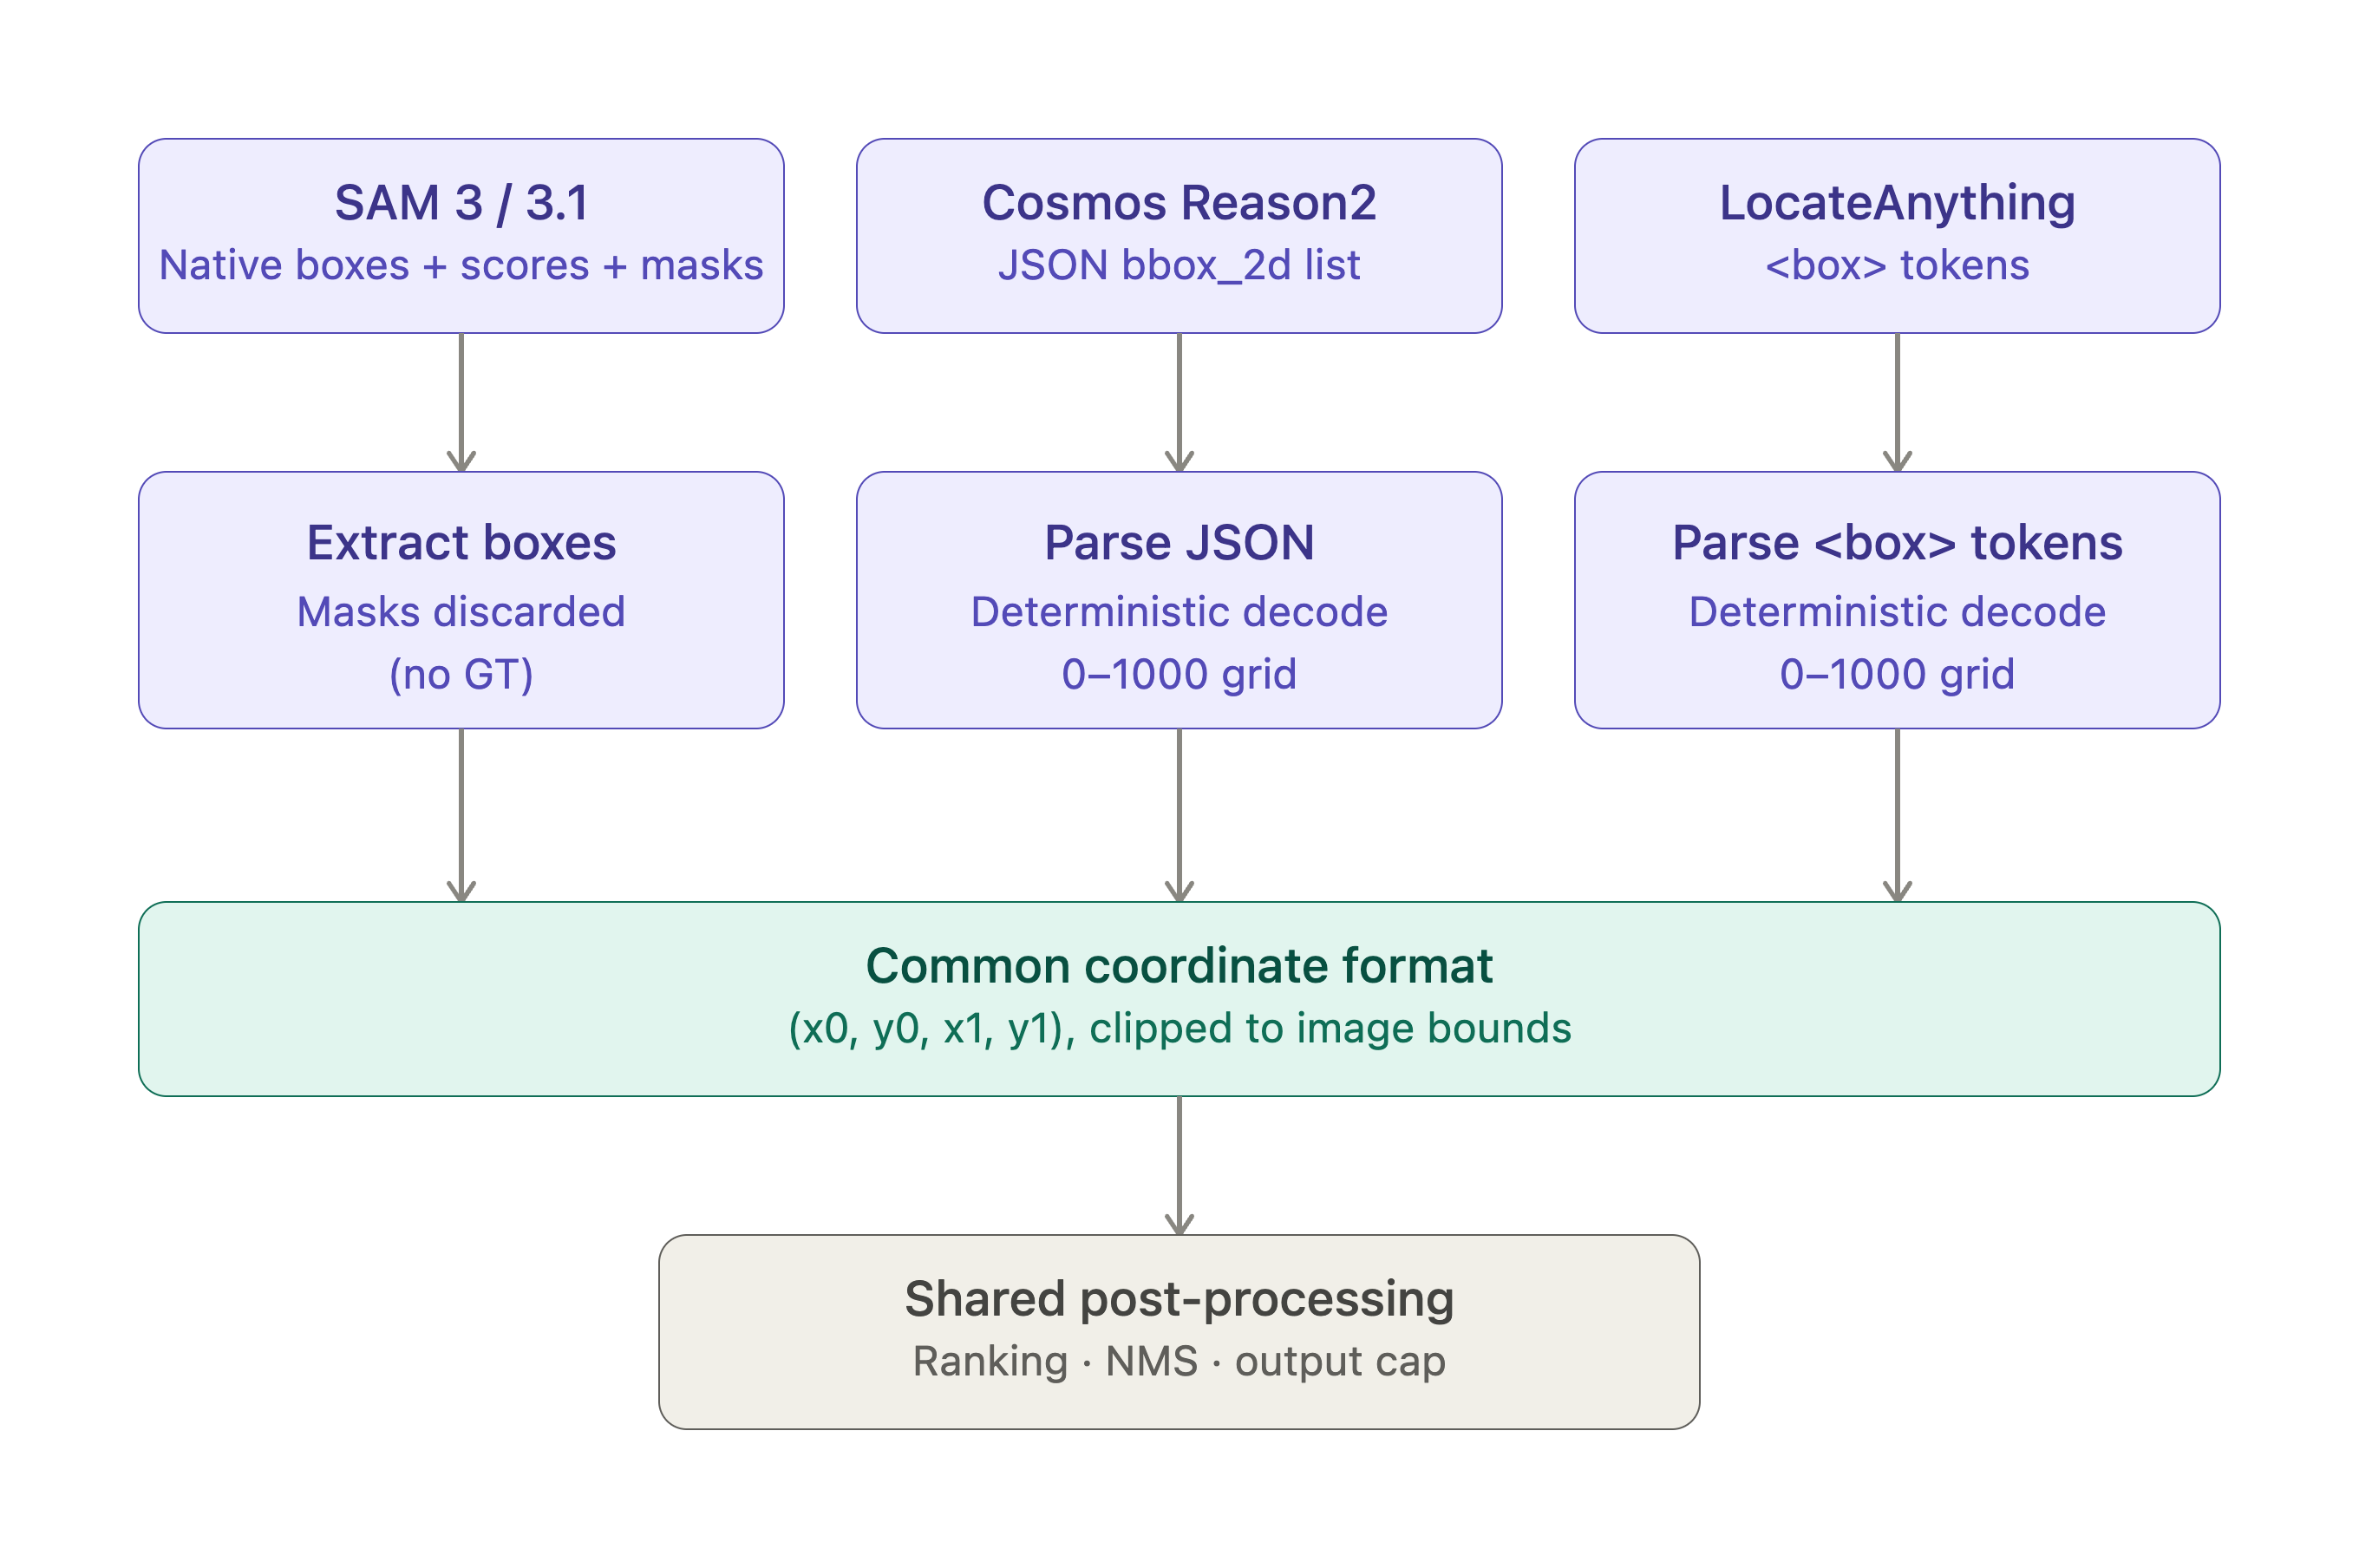
\includegraphics[width=\textwidth]{figures/prediction-normalisation-pipeline.png}
    \caption{Normalisation of model-specific outputs to a common coordinate format.}
    \label{fig:prediction-normalisation-pipeline}
\end{figure}

\newpage
\noindent Each inference call constituted a single semantic query, so \gls{NMS} was applied class-agnost\-ically, ranking predictions by confidence where available prior to suppression and output limiting. As LocateAnything and Cosmos Reason2 provide no per-box confidence, their predictions received a uniform score of \(1.0\), with stable sorting preserving generation order, leaving confidence-ranked \gls{AP} directly interpretable only for \gls{SAM}~3 and 3.1 and cross-model comparison reliant instead on the fixed-operating-point measures defined in Chapter~\ref{ch:evaluation}.

\subsection{Inference Execution and Runtime Measurement}
\label{sec:inference-execution}
Inference was process-isolated to bound memory use and provide a reliable recovery boundary between runs. Each \gls{SAM} model--prompt combination was executed in a fresh worker process over the complete evaluated image set. LocateAnything-3B used fresh workers for successive chunks of up to 64 images, whereas Cosmos Reason2 used smaller eight-image chunks to constrain \gls{RAM} and \gls{VRAM} growth. Each worker loaded the required model, persisted its predictions and completion status, and then terminated, making process exit the principal memory-cleanup boundary.

Model-specific input resizing was applied only where required by the inference architecture. LocateAnything images with a longest side exceeding 1536 pixels were downscaled before inference. Cosmos Reason2 used checkpoint-specific maximum sides of 2560 pixels for the 2B model and 1536 pixels for the 8B model. Source images remained unchanged, with localisation outputs mapped to their original image dimensions for evaluation.

Completed chunks and model--prompt combinations were reused only when their stored experimental fingerprint matched the active configuration, including the protocol and dataset hashes, model, prompt text, target classes, split, detection limits and evaluation thresholds. Incompatible stored results were rejected, allowing interrupted evaluations to resume without mixing predictions generated under different experimental settings.

Reported localisation latency was measured per image around the complete prediction call after source-image loading. Model initialisation, worker creation, image loading and result persistence were therefore excluded. The measurement included model-specific preprocessing, prompt preparation, inference or generation, output parsing, coordinate conversion, prediction filtering and \gls{NMS}. Reported latency consequently represents end-to-end prediction-pipeline latency rather than neural-network forward-pass time alone.

\newpage
\subsection{Taxonomy-Aware Ground-Truth Mapping}
\label{sec:prompt-matching}

The semantic mappings introduced in Subsection~\ref{sec:prompt-inventory} were formalised so that each query was evaluated only against the classes it was intended to retrieve. For prompt \(q\), let \(\mathcal{C}_q\) denote its predefined set of eligible classes. For image \(i\), the corresponding target \gls{GT} set was defined as:

\begin{equation}
G_i^{(q)} =
\left\{
g \in G_i :
\mathrm{class}(g) \in \mathcal{C}_q
\right\}.
\end{equation}

\noindent Annotations outside \(\mathcal{C}_q\) remained present as non-target objects, while images containing no eligible targets were retained so that erroneous predictions in target-absent scenes remained measurable. Unmatched predictions overlapping a non-target annotated object at \(\mathrm{IoU} \geq 0.50\) remained \glspl{FP}, but were recorded separately by non-target class to distinguish semantic confusion from predictions occurring on background or unannotated regions. 

\subsection{Controlled Prompt-Sensitivity Experiment}
\label{sec:prompt-sensitivity}
A controlled experiment examined the sensitivity of prompt-based localisation to changes in linguistic formulation. Unlike the broader and synonym-comparison queries used in the primary evaluation, all prompts within a sensitivity family shared the same target \gls{GT} set, with only their wording varied. Differences in localisation performance within a family could therefore be attributed more directly to prompt formulation rather than to changes in target-class scope.

Nine target families were evaluated: four from the \gls{MDWD}, corresponding to \emph{Mixed Waste}, \emph{Recyclable Material}, \emph{Organic Waste} and \emph{Orange \gls{CMD}}, and five from the \gls{MTSD}, corresponding to \emph{Pedestrian Crossing}, \emph{Stop Sign}, \emph{Roundabout Ahead}, \emph{No Entry (One Way)} and \emph{Blind-Spot Mirror(Convex Mirror)}. Each family contained four formulations designed to vary the linguistic expression of the query while preserving the same underlying target concept. The formulation types and their intended distinction are summarised in Table~\ref{tab:prompt-sensitivity-types} using \emph{Mixed Waste} as an illustrative example.

Within each family, all four formulations shared an identical target-class set and were evaluated on the same canonical test split. The protocol additionally verified identical positive-image, negative-image and target-box counts across variants, ensuring that observed differences reflected changes in prompt wording rather than changes in evaluation scope. The complete prompt inventory is provided in Appendix~\ref{app:prompt-sensitivity-prompts}.

The heterogeneous \emph{Other Waste} category was excluded because it represents a residual class for which a coherent set of semantically equivalent prompts could not be defined. Similarly, \emph{one way sign} was retained only within the synonym-comparison analysis because it is not a controlled paraphrase of \emph{no entry sign}.

\begin{table}[H]
\centering
\small
\caption{Prompt formulation types used in the prompt-sensitivity experiment.}
\label{tab:prompt-sensitivity-types}
\renewcommand{\arraystretch}{1.25}
\begin{tabularx}{\textwidth}{
    @{}
    >{\raggedright\arraybackslash}p{3.2cm}
    >{\raggedright\arraybackslash}X
    >{\raggedright\arraybackslash}p{5.0cm}
    @{}
}
\toprule
\textbf{Variant} & \textbf{Purpose} & \textbf{Example: Mixed Waste} \\
\midrule

Canonical
& Concise noun phrase used in the primary prompt inventory.
& \texttt{"Black garbage bag"} \\

Lexical paraphrase
& Rephrases the concept using alternative but semantically related terminology.
& \texttt{"Black refuse bag"} \\

Descriptive paraphrase
& Expresses the target through a fuller visual or semantic description.
& \texttt{"Black bag containing mixed household waste"} \\

Instruction
& Reformulates the same target as an explicit localisation request.
& \texttt{"Find all black mixed-waste bags"} \\

\bottomrule
\end{tabularx}
\end{table}

\noindent For each model and target family, precision, recall, \(F_1\) and mean matched-box \gls{IoU} were calculated independently for all four formulations. Prompt sensitivity was characterised using the mean, population standard deviation, minimum, maximum and range of each metric across the four variants. Absolute \(F_1\) variation was defined as:

\begin{equation}
\Delta F_1 =
\max(F_1) - \min(F_1),
\end{equation}

\noindent with relative degradation defined as:

\begin{equation}
\Delta F_{1,\mathrm{rel}} =
\frac{\max(F_1)-\min(F_1)}
{\max(F_1)}.
\end{equation}

\noindent Where all four formulations produced \(F_1=0\), relative degradation was set to zero for numerical completeness and interpreted as consistent failure rather than prompt robustness. The analysis additionally retained the best- and worst-performing formulations, the canonical and instruction-style \(F_1\) scores, and each non-canonical variant's deviation from the canonical \(F_1\).

Prompt stability was assessed independently of \gls{GT} through all six pairwise comparisons among the four prediction sets within each family. Predicted boxes were greedily matched at \(\mathrm{IoU}=0.50\). For two prediction sets containing \(N_A\) and \(N_B\) boxes, with \(M\) matched pairs, pairwise agreement was defined as:

\begin{equation}
F_{1,\mathrm{pair}} =
\frac{2M}{N_A+N_B},
\qquad
J_{\mathrm{pair}} =
\frac{M}{N_A+N_B-M}.
\end{equation}

\noindent Mean \gls{IoU} across matched prediction pairs and unmatched-box counts were also retained. Two empty prediction sets were treated as fully consistent, with \(F_{1,\mathrm{pair}}=J_{\mathrm{pair}}=1\). These consistency measures quantify stability in model output rather than localisation correctness and are therefore interpreted alongside the corresponding \gls{GT}-based performance measures.

\section{Multi-Attribute Traffic-Sign Classification}
\label{sec:attr-cls}
The third experimental track evaluates the transferability of pretrained visual representations to the four object-level attributes defined for the \gls{MTSD}, formulated as a multi-task classification problem in which each \gls{GT} traffic-sign crop is encoded once by a shared visual backbone and passed to four independent classification heads. Each head performs single-label classification within its respective attribute space, avoiding the sparse combinatorial label space that would result from treating every attribute combination as a separate class, while allowing the shared representation to support related visual cues across tasks.

Attribute classification uses the final \gls{QA}-approved \gls{MTSD} annotations, partitioned and cropped as described in Subsections~\ref{sec:md-partitioning} and~\ref{sec:md-augmentation-attribute}. Instances whose original \gls{GT} bounding box measured fewer than 20 pixels along either dimension were excluded because the available visual information was considered insufficient for reliable attribute recognition. This removed 1,256 of the 20,509 annotated instances, producing a fixed experiment-ready manifest of 19,253 crops: 15,465 for training, 1,898 for validation and 1,890 for testing. All retained crops contain valid supervision for the four modelled attributes, and the same manifest was used throughout the representation and adaptation experiments.

\subsection{Visual Representations and Experimental Design}
\label{sec:attribute-backbones}
Four pretrained visual-representation families were selected to span different architectural and pre-training paradigms. \gls{DINO}v3, \gls{VJEPA}~2.1 and LingBot-Vision use \gls{VIT}-based architectures, whereas ConvNeXt provides a convolutional counterpart pretrained through supervised ImageNet-1K classification. Base (-B) and Large (-L) configurations were evaluated for each family, allowing model capacity to be considered alongside representation type and adaptation strategy, as summarised in Table~\ref{tab:attribute-backbone-matrix}.

The experimental matrix comprises 18 principal configurations, comprising frozen linear probing and \gls{LoRA} adaptation for both capacities of all four families, together with full \gls{FT} for ConvNeXt-B and ConvNeXt-L. Full \gls{FT} was not evaluated for the \gls{VIT}-based families, as the memory requirements of end-to-end adaptation exceeded the practical limits of the available training hardware. The experiment therefore compares feasible representation--adaptation combinations rather than a fully crossed architecture-by-adaptation factorial design.

\begin{table}[H]
\centering
\caption{Representation families and adaptation strategies for multi-attribute traffic-sign classification.}
\label{tab:attribute-backbone-matrix}
\renewcommand{\arraystretch}{1.3}
\small
\begin{tabularx}{\textwidth}{
    @{}
    >{\raggedright\arraybackslash}p{2.6cm}
    >{\centering\arraybackslash}p{2.1cm}
    >{\centering\arraybackslash}p{2.1cm}
    >{\centering\arraybackslash}p{1.5cm}
    >{\centering\arraybackslash}p{1.5cm}
    >{\centering\arraybackslash}p{1.8cm}
    >{\centering\arraybackslash}p{1.8cm}
    @{}
}
\toprule
& \multicolumn{2}{c}{\textbf{Capacity}} & \multicolumn{3}{c}{\textbf{Adaptation Strategy}} & \\
\cmidrule(lr){2-3}\cmidrule(lr){4-6}
\textbf{Family} & \textbf{Base} & \textbf{Large} & \textbf{Frozen} & \textbf{\gls{LoRA}} & \textbf{Full \gls{FT}} & \textbf{Input Size} \\
\midrule
\gls{DINO}v3
& \gls{VIT}-B/16 & \gls{VIT}-L/16
& \checkmark & \checkmark & --
& \(224\times224\) \\
\gls{VJEPA}~2.1
& \gls{VIT}-B/16 & \gls{VIT}-L/16
& \checkmark & \checkmark & --
& \(384\times384\) \\
ConvNeXt
& Base & Large
& \checkmark & \checkmark & \checkmark
& \(224\times224\) \\
LingBot-Vision
& \gls{VIT}-B/16 & \gls{VIT}-L/16
& \checkmark & \checkmark & --
& \(224\times224\) \\
\bottomrule
\end{tabularx}
\end{table}

\subsubsection{Model Initialisation and Feature Extraction}
\label{sec:attrcls-initialisation}
All backbones were initialised from publicly released pretrained weights rather than trained from random initialisation. \gls{DINO}v3\footnote{\url{https://github.com/facebookresearch/dinov3}} was loaded through Hugging Face \texttt{transfo\-rmers} using the corresponding \texttt{facebook/dinov3-*-pretrain-lvd1689m} checkpoints. Its pooled CLS representation---\texttt{pooler\_output} where provided by the implementation,
otherwise the first output token---was used as the crop-level feature vector. \gls{VJEPA}~2.1\footnote{\url{https://github.com/facebookresearch/vjepa2}} was loaded through Meta's official \texttt{torch.hub} entry points and released \gls{VJEPA}~2.1 checkpoints, with fallback to \gls{VJEPA}~2.0 explicitly disabled; its encoder output tokens were mean-pooled to obtain a single crop-level representation. LingBot-Vision\footnote{\url{https://github.com/robbyant/lingbot-vision}} was loaded through the official \texttt{lingbot\_vision} interface, with normalised patch-token representations mean-pooled.  ConvNeXt-B and ConvNeXt-L\footnote{\url{https://pytorch.org/vision/stable/models/convnext.html}} were initialised directly thro\-ugh torchvision's corresponding model implementations with \texttt{IMAGENET1K\_V1} pretrained weights, applying global average pooling to the final spatial feature map.

As \gls{VJEPA}~2.1 is pretrained for video input, each static \gls{MTSD} crop was repeated along the temporal dimension to form a two-frame pseudo-clip matching the model's tubelet size. This satisfies the expected temporal input structure without introducing synthetic motion or additional visual information, allowing the video-pretrained representation to be evaluated within the same static-image classification framework as the image-based backbones. In every case, the resulting crop-level representation was supplied to the four attribute-specific classification heads, with model identifiers, loader backends, feature dimensions and parameter counts retained throughout for reproducibility.

\subsection{Adaptation Strategies}
\label{sec:attribute-adaptation}
Three adaptation regimes were implemented to vary the extent to which the pretrained representation was modified during transfer. In the frozen setting, all backbone parameters remained fixed and the backbone was retained in evaluation mode throughout training, such that optimisation was restricted to the four newly initialised classification heads. This provides a direct assessment of the separability of the target attributes using the pretrained representation without altering its underlying feature space.

Under \gls{LoRA} adaptation, the original backbone weights likewise remained frozen, while low-rank adapters and the classification heads were jointly optimised. All \gls{LoRA} configurations used rank \(r=8\), scaling factor \(\alpha=16\), dropout of 0.05 and \texttt{bias="none"}, ensuring that no pretrained backbone bias terms were updated. Adapter placement followed the internal structure of each backbone: \gls{DINO}v3 targeted the separate attention \texttt{q\_proj} and \texttt{v\_proj} transformations, whereas \gls{VJEPA}~2.1 and LingBot-Vision targeted their fused \texttt{qkv} projections. For ConvNeXt, adapters were inserted into the two pointwise linear layers of each block (\texttt{block.3} and \texttt{block.5} in the torchvision implementation), with target specifications applied to all matching modules in the loaded backbone and verified before optimisation to confirm correct insertion.

Full \gls{FT} was applied only to ConvNeXt-B and -L, for which both the pretrained backbone and the four classification heads were updated during optimisation. For every configuration, the parameter audit reported total and trainable parameters, while further separating trainable head and adapter parameters and recording the trainable proportion of the complete model. This enables the extent of task-specific adaptation to be considered alongside predictive performance.

\begin{figure}[H]
\centering
    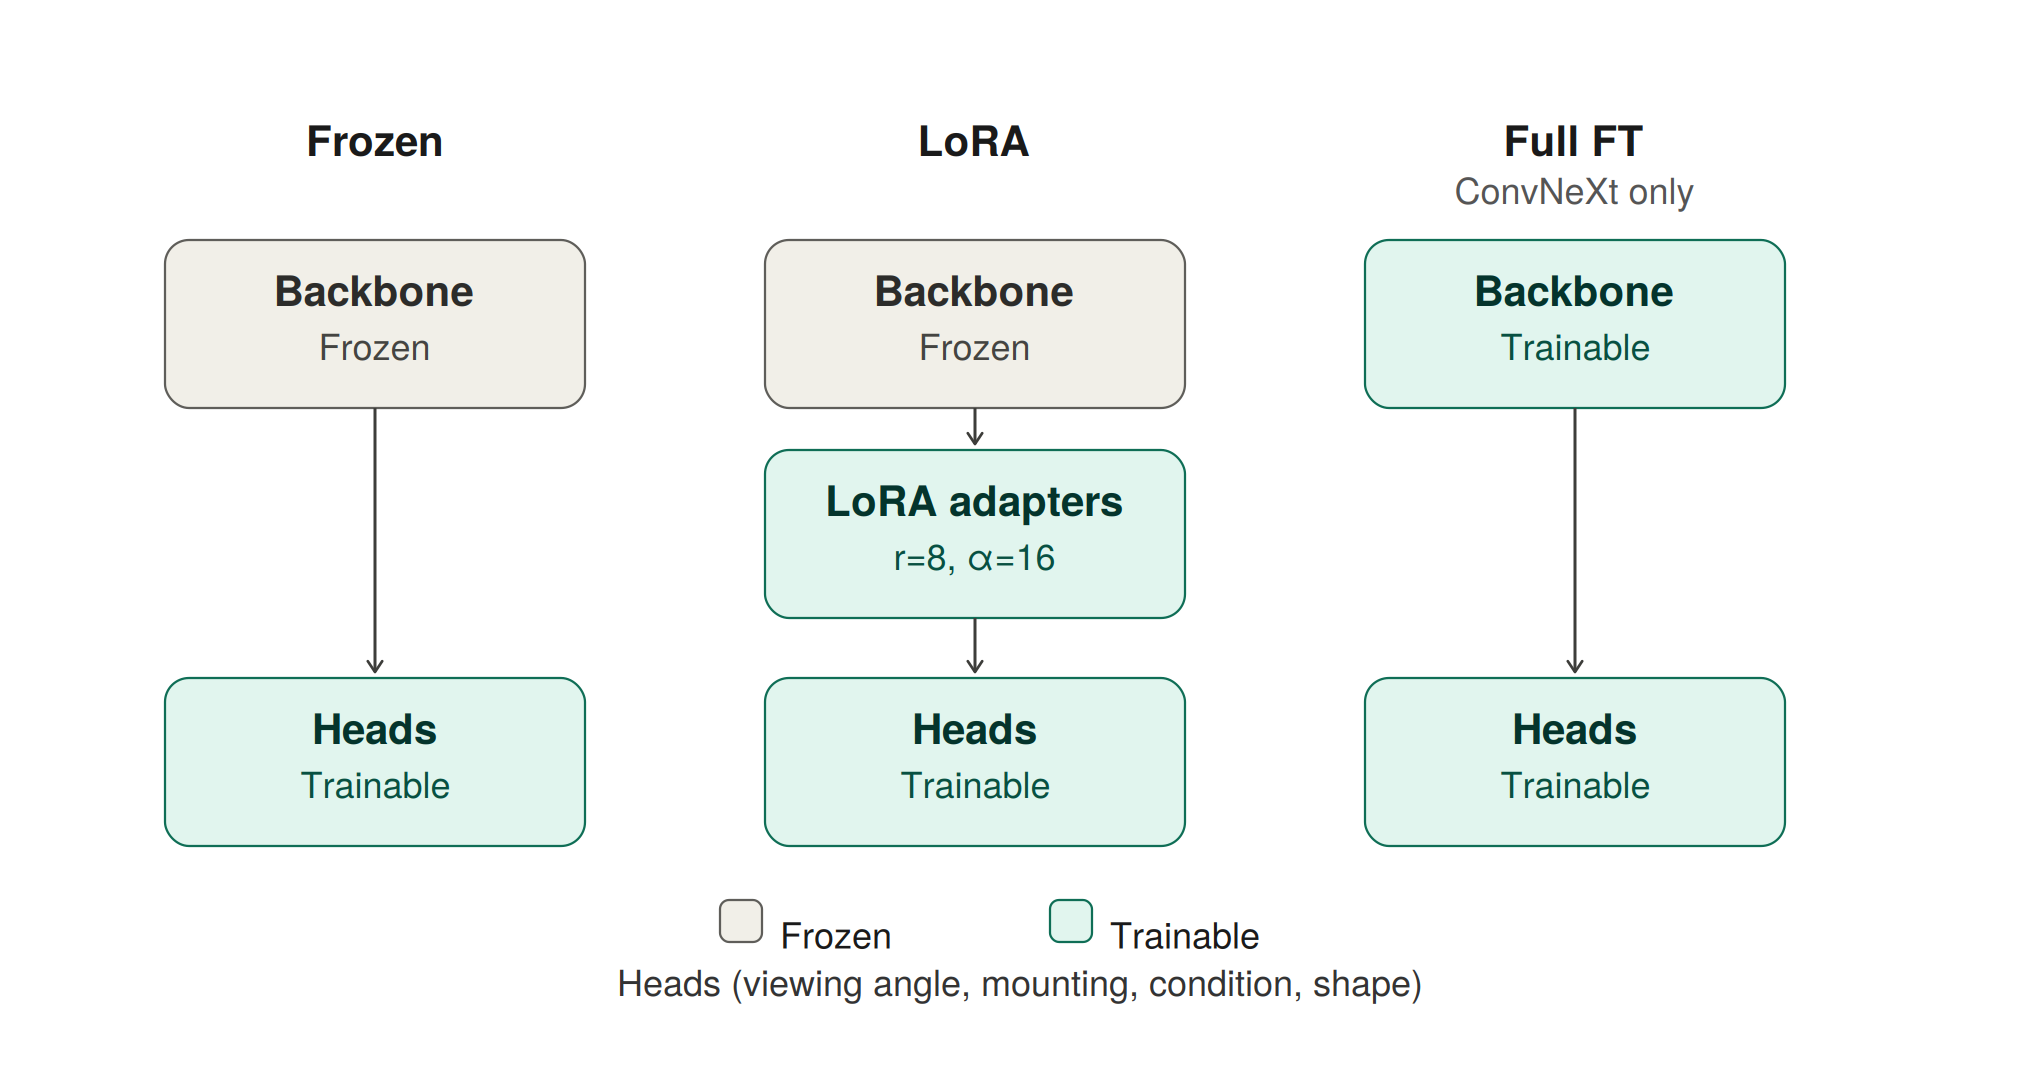
\includegraphics[width=0.95\textwidth]{figures/adaptation-strategies.png}
    \caption{Comparison of the three adaptation strategies evaluated for multi-attribute traffic-sign classification.}
    \label{fig:adaptation-strategies}
\end{figure}

\newpage
\subsection{Shared Multi-Head Architecture and Optimisation}
\label{sec:attribute-training}
Irrespective of backbone or adaptation strategy, the same downstream classification formulation was retained. For an input crop \(x\), the selected backbone \(f_{\theta}\) produces a pooled visual representation: 

\begin{equation}
\mathbf{z}=f_{\theta}(x),
\end{equation}

\noindent each attribute \(a\) is then predicted independently through a linear classification head,

\begin{equation}
\mathbf{o}_{a}
=
\mathbf{W}_{a}\mathbf{z}
+
\mathbf{b}_{a},
\end{equation}

\noindent where \(\mathbf{o}_{a}\) contains the logits for the classes belonging to attribute \(a\). The four heads share the backbone representation but contain no parameters in common with one another. This avoids four independent feature-extraction passes while retaining attribute-specific output spaces and loss functions. Class imbalance was addressed using weighted cross-entropy independently for each head. For class \(c\) within attribute \(a\), the class weight was calculated from the training partition as:

\begin{equation}
\label{eq:attr-class-weight}
w_{a,c}
=
\frac{N_a}{C_a n_{a,c}},
\end{equation}

\noindent where \(N_a\) denotes the number of training instances for attribute \(a\), \(C_a\) its number of classes and \(n_{a,c}\) the number of training instances belonging to class \(c\). This inverse-frequency formulation increases the contribution of less frequently represented classes while maintaining a frequency-weighted mean class weight of one within each task. For an instance with reference class \(y_a\), the loss for attribute \(a\) is:

\begin{equation}
\mathcal{L}_{a}
=
-w_{a,y_a}
\log p_{a,y_a},
\end{equation}

\noindent where \(p_{a,y_a}\) denotes the predicted probability assigned to the reference class. The overall optimisation objective is the unweighted sum of the four attribute losses, each term corresponding to its respective sign attribute:

\begin{equation}
\mathcal{L}_{\mathrm{joint}}
=
\mathcal{L}_{\mathrm{angle}}
+
\mathcal{L}_{\mathrm{mounting}}
+
\mathcal{L}_{\mathrm{condition}}
+
\mathcal{L}_{\mathrm{shape}}.
\end{equation}

\noindent Equal task weighting was retained so that no attribute received greater importance a priori, with class imbalance addressed independently within each head and no label smoothing applied. Per-head masking of missing labels was implemented as a defensive measure but never exercised, since the final manifest contains valid supervision for all four attributes.

\subsection{Training Procedure}
\label{sec:trainingprod}
A common optimisation protocol was applied across the 18 principal configurations to minimise procedural variation between representation families, model capacities and adaptation strategies. Shared settings and model- or adaptation-specific exceptions are summarised in Table~\ref{tab:attribute-training-config}.

\begin{table}[H]
\centering
\caption{Training configuration used for the multi-attribute classification experiments. Values are shared unless a model- or adaptation-specific exception is indicated.}
\label{tab:attribute-training-config}
\renewcommand{\arraystretch}{1.18}
\small
\begin{tabularx}{\textwidth}{
    @{}
    >{\raggedright\arraybackslash}p{5.0cm}
    >{\raggedleft\arraybackslash}X
    @{}
}
\toprule
\textbf{Setting} & \textbf{Configuration} \\
\midrule

Random seed
& 42 \\

Maximum epochs
& 150 \\

Optimiser
& AdamW \\

Weight decay
& 0.05 \\

Learning-rate schedule
& 5-epoch linear warm-up followed by cosine decay to zero \\

\addlinespace[0.35em]

Head learning rate
& \(1\times10^{-3}\) (frozen/\gls{LoRA}); \(4\times10^{-4}\) (full \gls{FT}) \\

\gls{LoRA} learning rate
& \(2\times10^{-4}\) \\

Fine-tuned backbone learning rate
& \(5\times10^{-5}\) \\

\addlinespace[0.35em]

DataLoader workers
& 4 \\

Effective batch size
& 32 \\

Physical batch size and accumulation
& \(32\times1\), or \(16\times2\) for variants requiring reduced physical batches \\

Gradient clipping
& Global norm \(=1.0\) \\

Mixed precision
& \gls{BF16} autocasting where supported \\

\addlinespace[0.35em]

Loss
& Class-weighted cross-entropy \\

Class weighting
& Per-attribute inverse-frequency weights calculated from the training split (Eq.~\ref{eq:attr-class-weight}) \\

Task weighting
& Equal weighting across all four heads \\

Missing labels
& Masked independently for the affected attribute head \\

\addlinespace[0.35em]

Early-stopping patience
& 10 epochs \\

Minimum improvement
& \(0.001\) validation mean macro-\(F_1\) \\

\bottomrule
\end{tabularx}
\end{table}

\newpage
\noindent Separate learning rates were assigned to the classification heads, \gls{LoRA} adapters and fully \gls{FT} backbone parameters to reflect their different initialisation states. Newly initialised heads therefore received larger updates, while pretrained backbone parameters were adapted more conservatively. Where the standard physical batch size exceeded available \gls{GPU} memory, gradient accumulation preserved an effective batch size of 32. Automatic batch-size reduction was disabled so that memory constraints could not silently alter the experimental configuration.

Checkpoint selection used validation mean macro-\(F_1\), calculated as the unweight\-ed mean of the four attribute-level macro-\(F_1\) scores. Early stopping was triggered after 10 consecutive epochs without an improvement exceeding \(0.001\), whereas checkpoint selection remained independent of this threshold, with any strict improvement updating the best checkpoint. Following training, only the checkpoint with the highest validation mean macro-\(F_1\) was evaluated on the held-out test partition.

These experiments were run on the same workstation used for the supervised \glspl{OD} and prompt-based localisation experiments. Python~3.11.15, PyTorch~2.11.0, \gls{CUDA} 12.8 and \gls{CUDNN}~9.19 were used, together with torchvision~0.26.0, Transformers~5.12.1, \gls{PEFT}~0.19.1, timm~1.0.27 and lingbot-vision~0.1.0. Python, NumPy and PyTorch \gls{CPU} and \gls{CUDA} random-number generators were seeded at 42. Configuration snapshots, dataset manifests, included group and split counts, class weights, checkpoints, evaluation outputs and the corresponding Git commit were retained for each run. Exact bitwise replication is not claimed, as \gls{CUDNN} autotuning, parallel data loading and mixed-precision operations were not constrained to fully deterministic execution.

\noindent\rule{\linewidth}{0.3pt}